% Options for packages loaded elsewhere
\PassOptionsToPackage{unicode}{hyperref}
\PassOptionsToPackage{hyphens}{url}
\documentclass[
  11pt,
]{article}
\usepackage{xcolor}
\usepackage[margin=22mm]{geometry}
\usepackage{amsmath,amssymb}
\setcounter{secnumdepth}{-\maxdimen} % remove section numbering
\usepackage{iftex}
\ifPDFTeX
  \usepackage[T1]{fontenc}
  \usepackage[utf8]{inputenc}
  \usepackage{textcomp} % provide euro and other symbols
\else % if luatex or xetex
  \usepackage{unicode-math} % this also loads fontspec
  \defaultfontfeatures{Scale=MatchLowercase}
  \defaultfontfeatures[\rmfamily]{Ligatures=TeX,Scale=1}
\fi
\usepackage{lmodern}
\ifPDFTeX\else
  % xetex/luatex font selection
\fi
% Use upquote if available, for straight quotes in verbatim environments
\IfFileExists{upquote.sty}{\usepackage{upquote}}{}
\IfFileExists{microtype.sty}{% use microtype if available
  \usepackage[]{microtype}
  \UseMicrotypeSet[protrusion]{basicmath} % disable protrusion for tt fonts
}{}
\makeatletter
\@ifundefined{KOMAClassName}{% if non-KOMA class
  \IfFileExists{parskip.sty}{%
    \usepackage{parskip}
  }{% else
    \setlength{\parindent}{0pt}
    \setlength{\parskip}{6pt plus 2pt minus 1pt}}
}{% if KOMA class
  \KOMAoptions{parskip=half}}
\makeatother
\usepackage{graphicx}
\makeatletter
\newsavebox\pandoc@box
\newcommand*\pandocbounded[1]{% scales image to fit in text height/width
  \sbox\pandoc@box{#1}%
  \Gscale@div\@tempa{\textheight}{\dimexpr\ht\pandoc@box+\dp\pandoc@box\relax}%
  \Gscale@div\@tempb{\linewidth}{\wd\pandoc@box}%
  \ifdim\@tempb\p@<\@tempa\p@\let\@tempa\@tempb\fi% select the smaller of both
  \ifdim\@tempa\p@<\p@\scalebox{\@tempa}{\usebox\pandoc@box}%
  \else\usebox{\pandoc@box}%
  \fi%
}
% Set default figure placement to htbp
\def\fps@figure{htbp}
\makeatother
\setlength{\emergencystretch}{3em} % prevent overfull lines
\providecommand{\tightlist}{%
  \setlength{\itemsep}{0pt}\setlength{\parskip}{0pt}}
\usepackage{bookmark}
\IfFileExists{xurl.sty}{\usepackage{xurl}}{} % add URL line breaks if available
\urlstyle{same}
\hypersetup{
  hidelinks,
  pdfcreator={LaTeX via pandoc}}

\author{}
\date{}

\ExplSyntaxOn
\cs_new:Npn \ReaderIfNativeAnchorTF #1 { \exp_args:Nx \str_if_in:nnTF {#1} {section*.} }
\ExplSyntaxOff
\makeatletter
\let\ReaderOriginalAnchorStart\hyper@anchorstart
\let\ReaderOriginalAnchorEnd\hyper@anchorend
\let\ReaderPendingAliases\@empty
\def\ReaderArmAliases#1{\gdef\ReaderPendingAliases{#1}}
\def\hyper@anchorstart#1{\ReaderIfNativeAnchorTF{#1}{\ReaderPendingAliases\global\let\ReaderPendingAliases\@empty}{}\ReaderOriginalAnchorStart{#1}}
\makeatother
\begin{document}

\section{Global boundary operators, compressed wave fronts, and normal
extension}\label{global-boundary-operators-compressed-wave-fronts-and-normal-extension}

\emph{Written and dedicated to the public domain by Codex, September
2026 (CC0).}

The local half-space calculus already tells us how a totally
characteristic operator acts near one boundary chart. On a manifold, the
same calculation must survive changes of coordinates, corners in the
operator kernel, and the distinction between an ordinary normal
derivative and a vector field tangent to the boundary. This lesson
builds that global calculus, proves its wave-front rules, and then uses
the exact boundary trace to extend solutions of noncharacteristic
equations. A final argument shows when conormal regularity is genuine
smoothness up to the boundary.

We keep the original Fourier convention \(D=-i\partial\), with inverse
factor \((2\pi)^{-n}\). A supported distribution is always represented
on the closed half-space; a restricted interior distribution is a
different object. Matrix products retain their input and output order.
All orders of symbols and conormal distributions are real unless a
theorem specifies an integer normal order.

The named prerequisites are
\href{conormal-transmission.pdf}{Singularities along a submanifold and
smooth boundary passage},
\href{totally-characteristic-operators.pdf}{Totally characteristic
operators on the half space}, \href{euclidean-symbol-calculus.pdf}{From
symbol estimates to operators on every Sobolev scale}, and
\href{geometric-microlocal-calculus.pdf}{Detecting regularity without
choosing coordinates}. The proofs below reproduce their particular
formulas when used, so the global construction remains readable from
these exact entry points.

\ReaderArmAliases{\ReaderOriginalAnchorStart{AN03-GBD-001}\ReaderOriginalAnchorEnd\begingroup\expandafter\def\csname @currentHref\endcsname{AN03-GBD-001}\label{AN03-GBD-001}\endgroup\ReaderOriginalAnchorStart{1-stretched-kernels-and-compressed-covectors}\ReaderOriginalAnchorEnd\begingroup\expandafter\def\csname @currentHref\endcsname{1-stretched-kernels-and-compressed-covectors}\label{1-stretched-kernels-and-compressed-covectors}\endgroup}
\subsection{1. Stretched kernels and compressed
covectors}\label{stretched-kernels-and-compressed-covectors}

\subsubsection{1.1. The real projective
blowup}\label{the-real-projective-blowup}

Let \(Y\) be a smooth embedded submanifold of codimension \(k\ge1\) in
\(X\). In coordinates \((z,y)\), \(Y=\{y=0\}\), \(y\in\mathbb R^k\).
Replace the normal origin by its lines: \[
 \{(z,L,v):L\in\mathbb{RP}^{k-1},\ v\in L\},
 \qquad \beta(z,L,v)=(z,v).
 \tag{GL1}
\] Here \(v\) is the actual normal vector, with both signs. Equivalently
the model is \((z,s,\omega)\), \(\omega\in S^{k-1}\), modulo
\((s,\omega)\sim(-s,-\omega)\), with \(v=s\omega\). For the chart in
which the \(i\)-th component of the line is nonzero, represent that line
by a vector \(w\) with \(w_i=1\). Coordinates are \((z,s,w_j:j\ne i)\),
and \(y=s w\). On overlaps, \[
 s_j=s_i w_j,\qquad w_\ell^{(j)}=w_\ell^{(i)}/w_j^{(i)} .
 \tag{GL2}
\] These are smooth invertible changes where \(w_j\ne0\), including
\(s_i=0\). They give a smooth manifold; the exceptional set is its
projectivized normal bundle, and the projection is a diffeomorphism away
from \(Y\). For \(k=1\), there is one line and the local projection is
the identity.

To prove independence of coordinates, let \(\bar y(z,y)\) be another
normal coordinate system vanishing on \(Y\). Hadamard's formula gives \[
 \bar y(z,y)=A(z,y)y,\qquad
 A(z,y)=\int_0^1\partial_y\bar y(z,\lambda y)\,d\lambda ,
 \quad A(z,0)\in GL(k,\mathbb R).
 \tag{GL3}
\] In a chart \(y=s w\), choose an index \(j\) for which
\((A(z,0)w)_j\ne0\). The new coordinates are \(\bar s=s(A(z,s w)w)_j\),
\(\bar w_\ell=(A(z,s w)w)_\ell/(A(z,s w)w)_j\), and the actual
transformed tangential coordinate \(\bar z(z,s w)\). The denominator
stays nonzero locally; all these functions are smooth at \(s=0\). The
inverse coordinate change has the same construction. The maps agree away
from the exceptional set, and therefore everywhere by continuity, so
their cocycle identities hold. This proves coordinate independence and
identifies the exceptional transition with the actual normal derivative.

If \(f,g\) vanish on \(Y\), their pullbacks have the form \(sF,sG\) by
the same integral formula. Wherever the normal derivative of \(g\) on
the line is nonzero, \(G(z,0,w)\ne0\), and \(f/g=F/G\) extends smoothly.
These ratio charts are thus intrinsic. No positive-ray quotient replaces
the projective quotient in this construction.

\subsubsection{1.2. The positive corner and its exact
coordinates}\label{the-positive-corner-and-its-exact-coordinates}

For boundary charts on two manifolds, keep \(x_n,y_n\ge0\) and their
positive normal rays. The projective interior normal cone at the corner
is \((\mathbb R_+^2\setminus\{0\})/\mathbb R_{>0}\). Its coordinate and
the radial coordinate are \[
 t=\frac{x_n+y_n}{2},\qquad
 r=\frac{2(x_n-y_n)}{x_n+y_n},\qquad
 x_n=t(1+r/2),\quad y_n=t(1-r/2),
 \quad t\ge0,\ -2\le r\le2 .
 \tag{GL4}
\] At \(t=0\), \(r\) records the ray; the projection collapses this
interval to the original corner. The two side faces are \(r=-2\), where
\(x_n=0\), and \(r=2\), where \(y_n=0\).

Boundary coordinate changes have normal parts \(\bar x_n=\alpha(x)x_n\),
\(\bar y_n=\gamma(y)y_n\), with \(\alpha,\gamma>0\). Set \(a=1+r/2\),
\(b=1-r/2\). Their exact lifted law is \[
 \bar t=\frac t2\,[\alpha(x)a+\gamma(y)b],\qquad
 \bar r=\frac{2[\alpha(x)a-\gamma(y)b]}
                  {\alpha(x)a+\gamma(y)b}.
 \tag{GL5}
\] The denominator is strictly positive on the entire closed interval:
\(a,b\ge0\), \(a+b=2\), and both coefficients are positive. The
tangential coordinates are the original coordinate changes evaluated at
\(x_n=t a,y_n=t b\). Thus the full lift is smooth up to every face and
corner, and its inverse is the lift of the inverse changes. It preserves
each side face and multiplies \(t\) by a smooth positive function. These
laws glue the stretched product intrinsically.

\begin{figure}
\centering
\pandocbounded{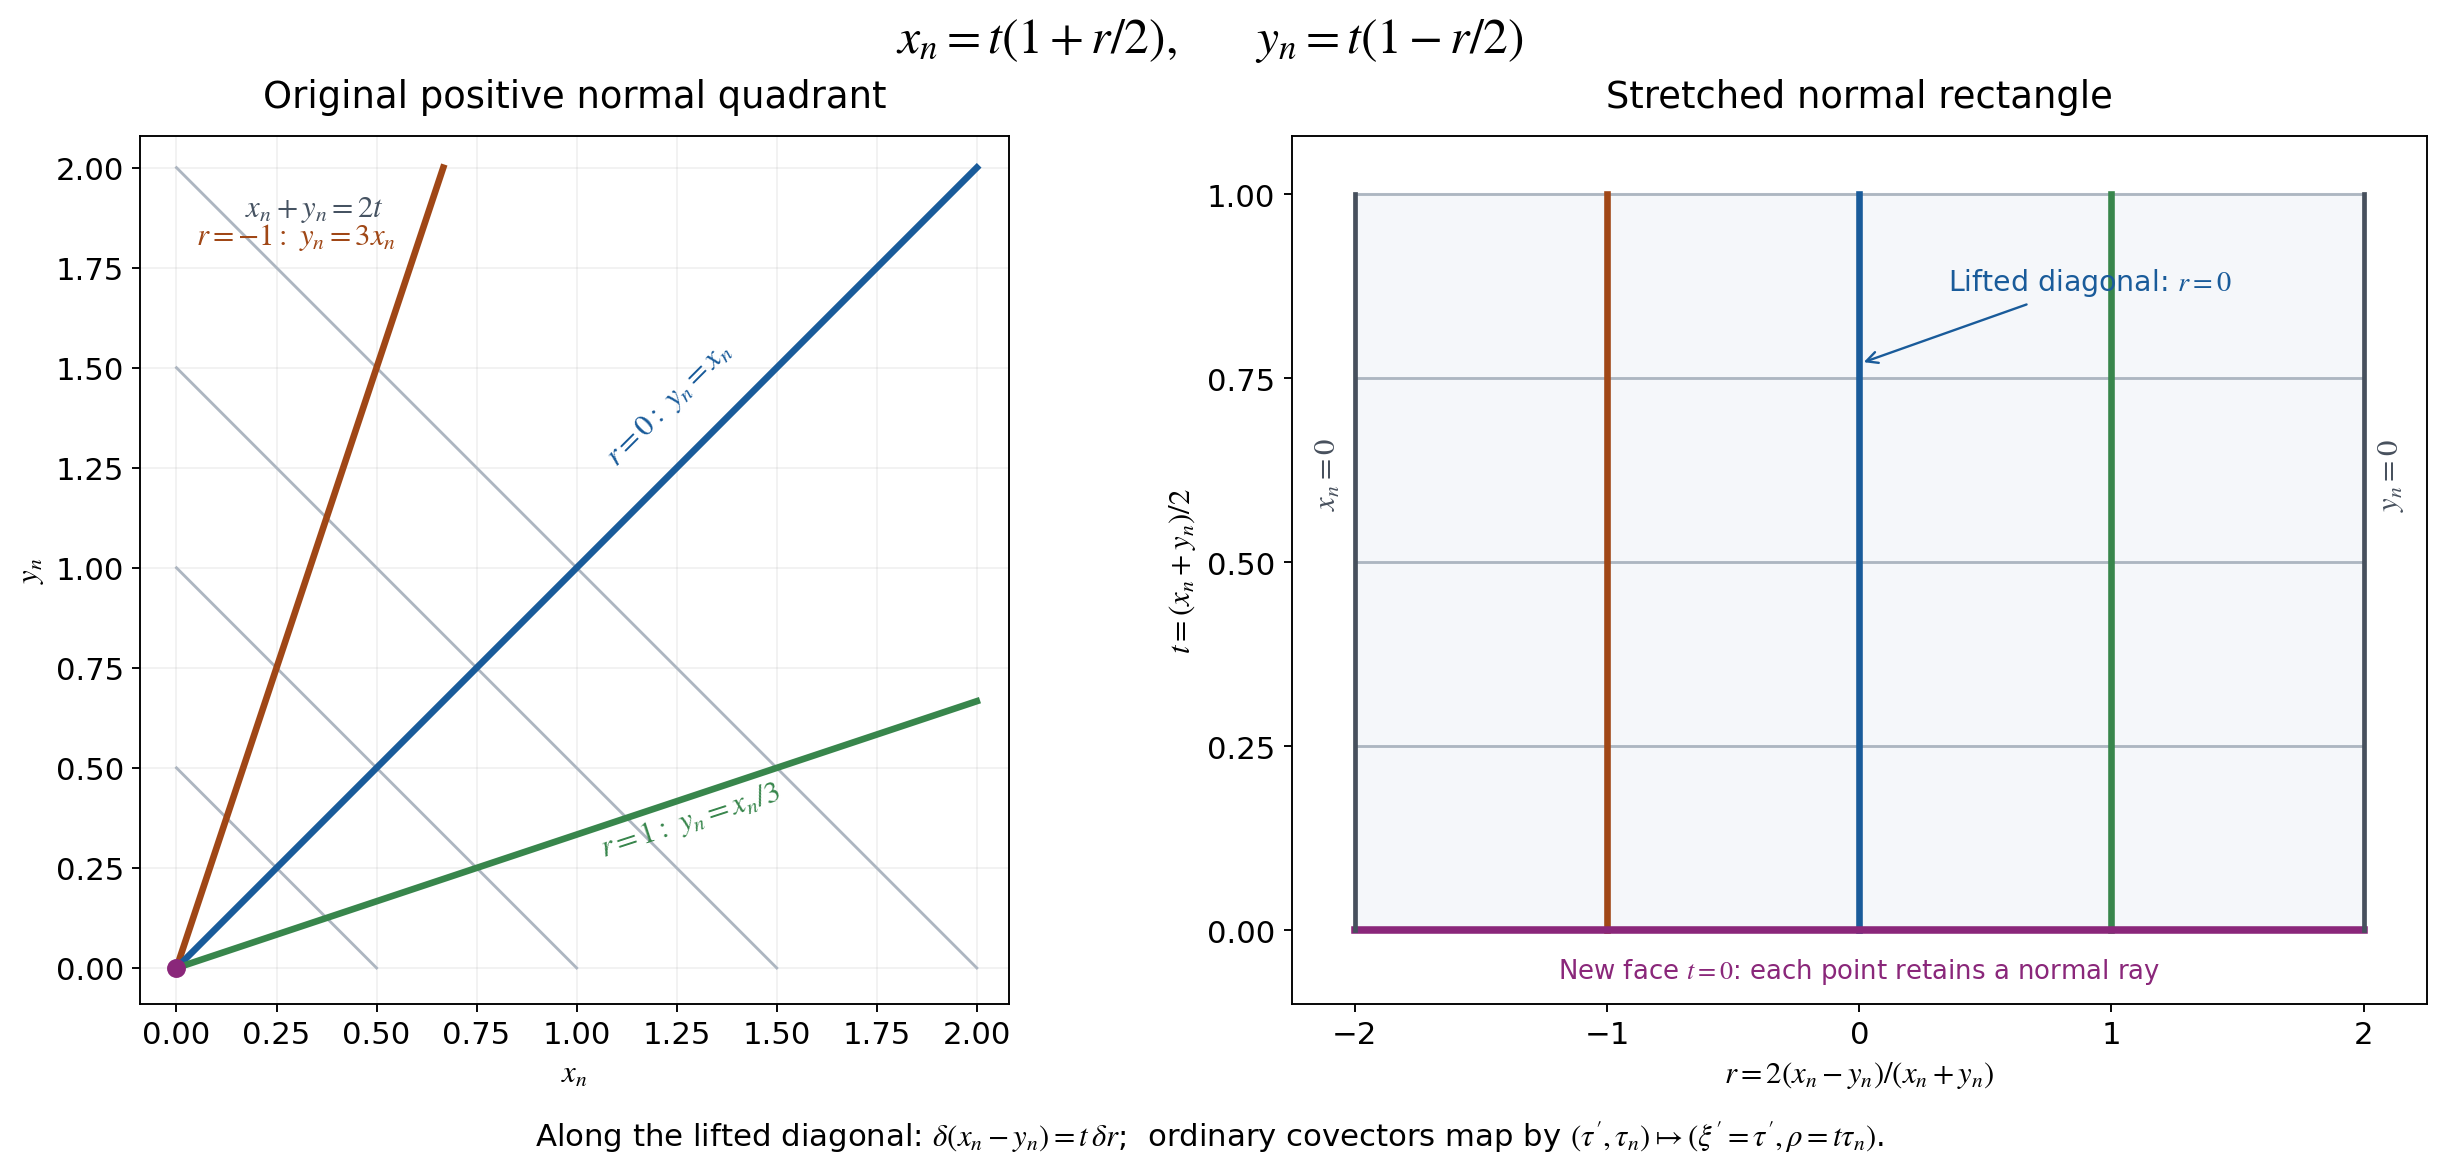
\includegraphics[keepaspectratio,alt={The original positive normal quadrant and its stretched rectangle}]{../figures/global_compressed_corner_geometry.png}}
\caption{The original positive normal quadrant and its stretched
rectangle}
\end{figure}

Figure GL-F1. The two panels retain the exact coordinates in (GL4). The
new face retains the ray when both normal variables vanish. The lifted
diagonal crosses that face. Only the two normal variables are drawn;
tangential coordinates and covectors retain their full dimensions in
(GL7)--(GL10). Reproducible source:
../figures/global\_compressed\_corner\_geometry.py.

For the square of one manifold the interior diagonal lifts to \[
 \widehat\Delta=\{x'=y',\ r=0,\ t\ge0\}.
 \tag{GL6}
\] The projection restricts to \((x',t)\mapsto(x',x_n=t)\), a
diffeomorphism with the original diagonal. The lifted diagonal avoids
\(r=\pm2\), and is transverse to \(t=0\) because its tangent includes
the \(t\) direction. This proves all these assertions at boundary points
as well as in the interior.

\subsubsection{1.3. The compressed bundle and both natural
maps}\label{the-compressed-bundle-and-both-natural-maps}

Pull \(N^*\widehat\Delta\) back by (GL6). In local coordinates its
covectors have the form \(\xi'\cdot d(x'-y')+\rho\,dr\). The normal
differential of the projection at the lifted diagonal is \[
 (\delta(x'-y'),\delta r)\longmapsto
       (\delta(x'-y'),\,t\,\delta r).
 \tag{GL7}
\] This follows by differentiating \(x_n-y_n=t r\) at \(r=0\). Dualizing
gives the natural map from the ordinary cotangent bundle: \[
 \lambda:T^*X\longrightarrow\widetilde T^*X,\qquad
 (\tau',\tau_n)\longmapsto(\xi'=\tau',\,\rho=x_n\tau_n).
 \tag{GL8}
\] It is an isomorphism for \(x_n>0\). At \(x_n=0\) its kernel is
precisely the ordinary conormal line to the boundary, and its image is
the hyperplane \(\rho=0\), canonically \(T^*\partial X\). The compressed
fibre itself still has dimension \(n\); its other covectors have not
been discarded.

The dual anchor is \[
 \widetilde TX\longrightarrow TX,\qquad
 (v',v_n)\longmapsto
       \sum_{j<n}v_j\partial_{x_j}+x_n v_n\partial_{x_n}.
 \tag{GL9}
\] Its smooth sections map bijectively onto smooth vector fields tangent
to the boundary. Indeed a tangent normal coefficient \(b(x',x_n)\)
vanishes at \(x_n=0\) and equals
\(x_n\int_0^1\partial_{x_n}b(x',s x_n)\,ds\). This constructs its smooth
inverse coefficient. Uniqueness follows in the interior and hence at the
boundary by continuity.

For an exact coordinate law write \(\bar x'=F(x',x_n)\),
\(\bar x_n=\alpha(x',x_n)x_n\), \(\alpha>0\). In the interior a
compressed covector is \(\xi'\cdot dx'+\rho\,dx_n/x_n\). Differentiating
the original coordinate functions, without dropping terms, gives \[
 \begin{aligned}
 \xi'&=(\partial_{x'}F)^T\bar\xi'
               +(\partial_{x'}\log\alpha)\bar\rho,\\
 \rho&=x_n(\partial_{x_n}F)^T\bar\xi'
               +(1+x_n\partial_{x_n}\log\alpha)\bar\rho .
 \end{aligned}
 \tag{GL10}
\] These expressions extend smoothly to the boundary. There their
determinant is \(\det\partial_{x'}F\ne0\); locally in the collar the
matrix is invertible, and its inverse is furnished by the inverse
boundary coordinate change. The law agrees with the pulled-back conormal
law in the interior by (GL7)--(GL8), and hence agrees everywhere. It
proves the intrinsic bundle identification, both anchors, and the
invariant hyperplane \(\rho=0\).

\subsubsection{1.4. The original symplectic form and
density}\label{the-original-symplectic-form-and-density}

In the interior substitute the full formula \(\tau_n=\rho/t\) into the
ordinary cotangent form \(\sum_j d\tau_j\wedge dx_j\). Since
\(d(\rho/t)=t^{-1}d\rho-\rho t^{-2}dt\), its exact expression is \[
 \omega=\sum_{j<n}d\xi_j\wedge dx_j+t^{-1}d\rho\wedge dt .
 \tag{GL11}
\] It is nondegenerate for \(t>0\). The \(t^{-1}\) factor is a boundary
singularity; there is no smooth symplectic form asserted there. In the
indicated order of coordinates, \[
 \frac{\omega^n}{n!}
 =(-1)^{n(n+1)/2}t^{-1}
       dx'\wedge dt\wedge d\xi'\wedge d\rho,\qquad
 |\omega^n/n!|^{1/2}
 =t^{-1/2}|dx'\,dt\,d\xi'\,d\rho|^{1/2}.
 \tag{GL12}
\] For the sign, move the original ordered pairs
\((d\xi_1,dx_1,\ldots,d\rho,dt)\) to the displayed base-then-fibre
order; the number of transpositions is \(n(n+1)/2\). The density law is
intrinsic because (GL11) was pulled from the original cotangent form.
Its singular factor remains explicit.

\subsubsection{1.5. The full stretched kernel for every symbol
order}\label{the-full-stretched-kernel-for-every-symbol-order}

Let \(a\in S_{\mathrm{la}}^m\), \(m\in\mathbb R\), in the local
half-space calculus. Keep its exact inverse Fourier distribution \[
 A(x,z)=(2\pi)^{-n}\int e^{iz\cdot\xi}a(x,\xi)\,d\xi,\qquad
 K(x,y)=x_n^{-1}
       A\left(x',x_n,x'-y',\frac{x_n-y_n}{x_n}\right)
       \quad(x_n>0).
 \tag{GL13}
\] Oscillatory integrals are defined by the cutoff-independent
distribution construction in (C4)--(C5). No residual assumption is made.
Differentiation in \(z\) raises the amplitude order by its exact degree;
integration by parts in \(\xi\) to a degree exceeding that order plus
\(n\) proves that \(A\) is smooth off \(z=0\), with arbitrary decay in
\(|z|\ge1\), uniformly with every base derivative on compact sets. Near
\(z=0\) its full phase and amplitude exhibit a conormal distribution of
order \(m\) by (C16), with ambient dimension \(2n\) and codimension
\(n\).

The Fourier support in the original definition implies
\(\operatorname{supp}_{z_n}A\subset(-\infty,1]\). In fact the partial
Fourier transform of \(a\) is supported in \([-1,\infty)\); inverse
transformation evaluates it at \(-z_n\), with the original inverse
Fourier factor. At \(z_n=1\) the distribution is already smooth, since
that point is away from \(z=0\). Its vanishing on \(z_n>1\) therefore
makes every derivative vanish on \(z_n=1\).

The determinant of (GL4) is \(-t\), so a kernel half-density pulls back
with coefficient \(k=t^{1/2}K\). Put \(H=t^{1/2}k=tK\). The entire
formula is {\footnotesize
\[
 k=t^{-1/2}(1+r/2)^{-1}
 A\left(x',t(1+r/2),x'-y',\frac{r}{1+r/2}\right),\qquad
 H=(1+r/2)^{-1}
 A\left(x',t(1+r/2),x'-y',\frac{r}{1+r/2}\right).
 \tag{GL14}
\]
} Thus both square-root factors, the normal Jacobian and the complete
argument of \(A\) are retained.

Near the lifted diagonal \(1+r/2>0\). In (GL13) change only the
integration variable \(\xi_n=(1+r/2)\rho\). Its positive Jacobian
cancels exactly the displayed \((1+r/2)^{-1}\), giving \[
 H=(2\pi)^{-n}\int
 e^{i[(x'-y')\cdot\xi'+r\rho]}\,
 a\bigl(x',t(1+r/2),\xi',(1+r/2)\rho\bigr)\,d\xi'\,d\rho .
 \tag{GL15}
\] The amplitude has all order-\(m\) estimates on compact base sets: an
\(r\)-derivative gives \(t\partial_{x_n}a/2\) or
\(\rho\partial_{\xi_n}a/2\); the latter has the original order \(m\). A
\(t\)-derivative has the bounded factor \(1+r/2\); frequency derivatives
lower the order normally. The same argument handles any iterated mixed
derivative. Equations (GL14) and (GL15) are exact descriptions of the
same kernel, not a substitution omitting a density factor. They prove
that \(H|dx'\,dy'\,dt\,dr|^{1/2}\) is conormal along \(\widehat\Delta\),
smooth in \(t\ge0\).

At \(r=2\), the last argument of \(A\) is \(1\), so the preceding
support argument gives side flatness, including all \(t\) and tangential
derivatives. At \(r=-2\), that argument tends to minus infinity. Its
derivatives and the displayed prefactor grow only as fixed powers of
\((2+r)^{-1}\). The arbitrary large-\(|z|\) decay absorbs each such
power, proving flatness there as well. These estimates are uniform for
compact \(t,x',y'\) ranges. Off \(\widehat\Delta\), the same Fourier
argument proves smoothness.

\subsubsection{1.6. The exact principal half-density and inverse
reconstruction}\label{the-exact-principal-half-density-and-inverse-reconstruction}

In the full amplitude of (GL15), the difference from its \(r=0\) value
is \[
 \frac r2\int_0^1
 [\,t\partial_{x_n}a+\rho\partial_{\xi_n}a\,]
 \bigl(x',t(1+s r/2),\xi',(1+s r/2)\rho\bigr)\,ds .
 \tag{GL16}
\] Retain this entire integral. Integration by parts in \(\rho\), using
\(r e^{ir\rho}=i^{-1}\partial_\rho e^{ir\rho}\), changes it to the exact
order-\((m-1)\) amplitude \[
 \frac i2\,\partial_\rho\int_0^1
 [\,t\partial_{x_n}a+\rho\partial_{\xi_n}a\,]
 \bigl(x',t(1+s r/2),\xi',(1+s r/2)\rho\bigr)\,ds .
 \tag{GL17}
\] A compact cutoff in \(r\) on this chart is independent of \(\rho\)
and does not change that calculation. The defining cutoff limit
justifies the integration by parts, by (C4)--(C5). Hence the principal
conormal half-density of \(H\), in the parametrization
\((x',x',t,0;\xi',-\xi',0,\rho)\), is precisely the class of \[
 a(x',t,\xi',\rho)\,|dx'\,dt\,d\xi'\,d\rho|^{1/2}
 \quad\pmod{\text{one lower amplitude order}} .
 \tag{GL18}
\] For \(k\), the additional \(t^{-1/2}\) is still present. Comparing
(GL18) with (GL12) makes its scalar coefficient \(a\) a principal symbol
on the compressed cotangent bundle. The full remainder is
(GL16)--(GL17); it has not been removed from the original kernel. The
coordinate invariance follows from the full determinant law (C19)--(C20)
and the actual conormal coordinate change (GL10). In the intrinsic
convention of (C21), the half-density in (GL18) has symbol order
\(m+n/2\): its fibre half-density has dilation degree \(n/2\). Dividing
the original principal half-density of \(k\) by (GL12) leaves the
ordinary scalar or matrix symbol order \(m\). Neither convention changes
the amplitude or the original operator.

Conversely, take a compactly supported conormal family \(H\) along
\(\widehat\Delta\), of this order and smooth parameter type, flat at
both side faces. For \(z_n<1\) its inverse kernel is \[
 A(x,z)=\frac{2}{2-z_n}
 H\left(x',x'-z',\,\frac{x_n(2-z_n)}2,\,
                         \frac{2z_n}{2-z_n}\right),\qquad
 A(x,z)=0\quad(z_n\ge1).
 \tag{GL19}
\] These are the inverse of the full coordinate and prefactor formulas,
not just their diagonal restrictions. Near \(z=0\), pull back an
oscillatory conormal amplitude for \(H\) by this smooth map. Its normal
phase is \(z'\cdot\xi'+[z_n/(1-z_n/2)]\rho\). The change
\(\rho=(1-z_n/2)\eta_n\) has positive Jacobian \(1-z_n/2\), which
cancels the prefactor \(1/(1-z_n/2)\) in (GL19). The resulting amplitude
has order \(m\) with all base derivatives, including \(x_n\), by the
same product and chain rules used for (GL15). Compact localization and
the full amplitude reduction (C5) therefore give a smooth
\(x\)-dependent inverse Fourier symbol of order \(m\), with all
finite-seminorm bounds.

Away from \(z=0\), (GL19) is smooth. Flatness at \(r=-2\) gives
arbitrary decay as \(z_n\to-\infty\): each \(x_n\)-derivative introduces
at most one additional power of \(2-z_n\), absorbed by another flatness
order. Flatness at \(r=2\) gives a smooth zero extension at \(z_n=1\).
Compact tangential support controls \(z'=x'-y'\); all these far
contributions are Schwartz in \(z\), uniformly with every
\(x\)-derivative. If \(H\) is supported in \(t\le T\), then \(A\) is
supported in \(x_n\le2T\), since \(x_n=t(1+r/2)\le2t\). Its base
derivatives thus have every original \((1+x_n)^{-\nu}\) estimate.

Define the exact symbol \[
 a(x,\xi)=\int e^{-iz\cdot\xi}A(x,z)\,dz .
 \tag{GL20}
\] The near contribution is order \(m\) by the preceding reduction and
the far contribution is residual. Since \(A=0\) for \(z_n>1\), \[
 \mathcal F_{\xi_n}a(x,\xi',s)
 =2\pi\int e^{-iz'\cdot\xi'}A(x,z',-s)\,dz',
 \qquad \operatorname{supp}_s\mathcal F_{\xi_n}a\subset[-1,\infty).
 \tag{GL21}
\] This proves lacunarity with its exact sign and Fourier constant. Thus
\(a\in S_{\mathrm{la}}^m\), and (GL13)--(GL15) recover the original
half-density kernel exactly. Fourier inversion proves uniqueness of the
symbol on \(x_n>0\), and smoothness in \(x_n\) gives uniqueness at zero.
This proves the compact local converse as well as the forward statement
for every real \(m\).

\subsubsection{1.7. The exact boundary
action}\label{the-exact-boundary-action}

Let \(u\) be smooth up to the boundary with compact support. Write
\(s=x_n>0\), \(a_r=1+r/2\). At fixed \(s\), the actual changes of
integration variables are \[
 y_n=s\frac{1-r/2}{1+r/2},\qquad
 t=s/a_r,\qquad |dy_n|=s a_r^{-2}|dr|,
 \qquad K(x,y)|dy_n|=a_r^{-1}H(x',y',s/a_r,r)|dr|.
 \tag{GL22}
\] Thus the full operator action, interpreted as a distributional
pairing at the diagonal, is \[
 (T_a u)(x',s)=\int_{-2}^{2}\int
 \frac{H(x',y',s/a_r,r)}{a_r}
 u\left(y',s\frac{1-r/2}{a_r}\right)\,dy'\,dr .
 \tag{GL23}
\] For a forward symbol, compactly localize the base variables on the
output region; (GL14) retains the same uniform side estimates there. For
an inverse kernel its given compact support provides this localization.
Choose a partition in \((x'-y',r)\) which is one near its origin and
supported away from \(r=\pm2\). On that part the smooth conormal family
and the compact smooth test function in (GL23) converge, with every
\(x'\) derivative, as \(s\) decreases to zero. Oscillatory formula
(GL15) justifies the convergence: integrate by parts in its normal base
variables to an order exceeding the amplitude order plus \(n\), exactly
as in (C4). The resulting integrable frequency majorant is uniform in
\(s\).

On the complementary part the kernel is a smooth function. Near
\(r=-2\), every \(s\), \(x'\) or integration-variable derivative of
(GL23) introduces only a fixed negative power of \(a_r\). The arbitrary
side-flatness order in (GL14) absorbs that power. Near \(r=2\), the same
statement follows from smooth flatness at that side. Away from those
sides all factors have ordinary compact smooth bounds. Dominated
convergence, including each derivative, proves the boundary limit \[
 \begin{aligned}
 (T_a u)(x',0)
 &=\int_{-2}^{2}\int a_r^{-1}H(x',y',0,r)u(y',0)\,dy'\,dr\\
 &=\int\!\int_{-\infty}^{1}
       A(x',0,x'-y',z_n)u(y',0)\,dz_n\,dy'\\
 &=(2\pi)^{-(n-1)}\int e^{ix'\cdot\xi'}
       a(x',0,\xi',0)\widehat{u(\cdot,0)}(\xi')\,d\xi'.
 \end{aligned}
 \tag{GL24}
\] The second equality uses the full change \(z_n=r/a_r\),
\(dz_n=a_r^{-2}dr\), and \(H(x',y',0,r)=a_r^{-1}A(x',0,x'-y',z_n)\). The
last equality is exact partial Fourier inversion at normal frequency
zero. The preceding localization and integration by parts justify both
equalities even when \(A\) is not a function at \(z=0\). When \(n=1\),
the tangential integrals have dimension zero and the factor is one. This
is the full boundary action, with all orders and all kernel factors, and
it agrees with the original jet formula (5.2) for \(k=0\).

\ReaderArmAliases{\ReaderOriginalAnchorStart{AN03-GBD-002}\ReaderOriginalAnchorEnd\begingroup\expandafter\def\csname @currentHref\endcsname{AN03-GBD-002}\label{AN03-GBD-002}\endgroup\ReaderOriginalAnchorStart{2-proper-global-operators-and-conormal-smoothing}\ReaderOriginalAnchorEnd\begingroup\expandafter\def\csname @currentHref\endcsname{2-proper-global-operators-and-conormal-smoothing}\label{2-proper-global-operators-and-conormal-smoothing}\endgroup}
\subsection{2. Proper global operators and conormal
smoothing}\label{proper-global-operators-and-conormal-smoothing}

\subsubsection{2.1. The global kernel and its actual
pushforward}\label{the-global-kernel-and-its-actual-pushforward}

Choose a smooth function \(t\) on the stretched square, positive off its
new face and vanishing simply on that face. Near a boundary diagonal
point it can be the original \((x_n+y_n)/2\). Define the order-\(m\)
class by kernels represented as \[
 k=t^{-1/2}H,\qquad
 H\in I^m(X\widehat\times X,\widehat\Delta;\Omega^{1/2}),
 \qquad H\text{ flat on both original side faces}.
 \tag{GC1}
\] Here conormality at the new face has precisely the smooth family
meaning specified before (GL1). A bundle kernel additionally has values
in \(\operatorname{Hom}(E_y,F_x)\). Multiplication by its smooth frame
changes is included in the conormal topology.

There is a well-defined pushforward despite the separate factor
\(t^{-1/2}\). Indeed, in the original normal chart, let a test
half-density have coefficient \(p(x,y)\). Its pullback has coefficient
\(t^{1/2}p(\beta(x',y',t,r))\), since the absolute normal determinant is
\(t\). Thus the actual pairing is \[
 \langle\beta_*k,p\rangle
 =\int_0^\infty
   \left\langle H(x',y',t,r),
       p(x',t(1+r/2),y',t(1-r/2))\right\rangle_{x',y',r}\,dt.
 \tag{GC2}
\] The conormal family is a smooth distribution-valued function of
\(t\). On a compact interval its pairing with the smooth compact test
family is bounded by finitely many test derivatives and symbol
seminorms, by (C4). The integral is consequently well defined and
continuous. The blowdown has compact projective fibres, so the inverse
image of a compact test support is compact; away from the corner it is a
diffeomorphism. Those facts reduce the general pairing to finitely many
such charts. Equation (GC2) is the complete meaning of pairing \(k\)
with the pulled-back test half-density. Neither square-root factor is
separately discarded, and no pairing of an arbitrary distribution with a
nonsmooth test coefficient is asserted.

If \(\bar t\) is another admissible defining function, Hadamard's
formula gives \(\bar t=c t\), with \(c>0\) smooth near the new face.
Away from that face both functions are positive. Hence \[
 \bar H=\bar t^{1/2}k=c^{1/2}H.
 \tag{GC3}
\] Multiplication by \(c^{1/2}\), and by its smooth inverse, preserves
the conormal class and side flatness. The kernel, its pairing and its
order are independent of this choice.

Every compactly localized kernel of (GC1) is the original half-space
kernel of a lacunary order-\(m\) symbol by (GL19)--(GL21). Away from the
lifted diagonal the localized resolved coefficient is smooth, and the
same inverse gives a residual symbol. The latter assertion also applies
between distinct boundary charts: coordinates in the two charts may be
used as the two independent tangential variables in the smooth kernel;
there is no conormal singularity to align. Near an actual diagonal point
use the same coordinate chart on both factors. Interior charts give the
ordinary conormal pseudodifferential kernel by (C18).

The local theorem on smooth inputs therefore proves a continuous map \[
 A:C_c^\infty(X;\Omega^{1/2}\otimes E)
       \longrightarrow C^\infty(X;\Omega^{1/2}\otimes F).
 \tag{GC4}
\] For fixed input support and a fixed output compact set, only finitely
many product charts occur. Each local estimate uses finitely many
derivatives of the input, and the sum of these estimates is finite. This
proves the stated LF-to-Fréchet continuity. Formula (GL24) supplies its
boundary value, and the original formula (5.2) supplies every normal
jet. Conversely the local quantizations have exactly (GC1) by
(GL13)--(GL18), so this kernel description and the patched local
definition determine the same class. We denote it by
\(\Psi_b^m(X;E,F)\).

To check coordinate invariance at all orders, the stretched coordinate
change is (GL5), its conormal change is (GL10), and its complete
amplitude and determinant are (C19). Reducing that entire amplitude by
(C5) gives the transformed symbol, with the full order-\((m-N)\)
remainder after \(N\) terms. All frequency factors created by a base
derivative pair with a frequency derivative and retain order \(m\). Thus
the operator class, not only its leading term, is coordinate invariant.
The local construction and the pushforward above agree in the interior
and then as distributions by the same conormal family pairing (GC2).

\subsubsection{2.2. The symbol quotient and actual realization of every
symbol}\label{the-symbol-quotient-and-actual-realization-of-every-symbol}

For a compressed symbol \(a\), the original principal half-density of
the kernel is the class of \[
 a(x',t,\xi',\rho)t^{-1/2}
       |dx'\,dt\,d\xi'\,d\rho|^{1/2}.
 \tag{GC5}
\] The singular half-density multiplying \(a\) is the invariant absolute
symplectic half-density in (GL12). The complete determinant law (C20)
therefore gives a scalar symbol, or a section of
\(\operatorname{Hom}(E,F)\), on \(\widetilde T^*X\), of ordinary order
\(m\), modulo order \(m-1\). Both (GL16) and (GL17) remain its actual
lower-order kernel remainder. Define \(S^m(\widetilde T^*X)\) using
every local compact base set, all base derivatives, and the frequency
bound \(\langle(\xi',\rho)\rangle^{m-|\alpha|}\). The fibre
transformation (GL10) and its inverse have smooth bounded coefficients
on each compact chart; the chain rule proves that this definition is
intrinsic. The leading symbol map has kernel exactly \(\Psi_b^{m-1}\),
by the local normal-form kernel assertion (C21).

We prove surjectivity while retaining the original prescribed symbol.
Choose a locally finite cover by precompact boundary or interior charts
\(U_j\), with locally finite closures. Choose a partition \(\varphi_j\)
with support in these charts and \(\psi_j\in C_c^\infty(U_j)\) equal to
one on a neighborhood of \(\operatorname{supp}\varphi_j\). For a given
symbol \(a\), compactly localize a full representative \(a_j\) in the
\(j\)-th frame so that it equals \(a\) on that neighborhood. In a
boundary chart take exactly the lacunary modification \[
 (a_j)_\rho(x,\xi)=\int a_j(x,\xi',\xi_n-v)\rho(v)\,dv,
 \quad \widehat\rho\in C_c^\infty((-1/2,1)),\quad
 \widehat\rho=1\text{ near }0.
 \tag{GC6}
\] Keep \(a_j=(a_j)_\rho+[a_j-(a_j)_\rho]\): the bracket is residual by
the full Taylor integral (4.8), and every original symbol seminorm
remains controlled. Quantize the first term and set \[
 A=\sum_j\varphi_j T_{(a_j)_\rho}\psi_j
 \tag{GC7}
\] in boundary charts, using ordinary quantization for interior charts.
The sum is locally finite and has order \(m\). Its two support
projections are proper: above a compact base set only finitely many
chart closures occur, and both factors in each term have compact support
in that chart. The leading term is \(\sum_j\varphi_j a=a\).
Multiplication on the input has its complete product remainder, of order
\(m-1\), from (8.3); \(\psi_j=1\) near the working diagonal. The
residual bracket in (GC6) has not become an equality between the
original full symbol and its modification; it is explicitly the error in
this realization. This gives both quotients \[
 \Psi_b^m/\Psi_b^{m-1}\simeq
 S^m(\widetilde T^*X)/S^{m-1}(\widetilde T^*X),
 \tag{GC8}
\] with the same isomorphism when the operator spaces are restricted to
proper support. The bundle version follows in the same charts, with the
actual frame transitions and (GC5).

\subsubsection{2.3. Proper composition, adjoints and all asymptotic
remainders}\label{proper-composition-adjoints-and-all-asymptotic-remainders}

Let \(A\in\Psi_b^m(X;F,G)\) and \(B\in\Psi_b^{m'}(X;E,F)\) be properly
supported. For every compact output set the support of \(A\) meets only
a compact set of intermediate variables, and that compact set meets only
a compact input set under \(B\). The reverse argument starts at a
compact input set. This proves proper support of the composed operator
and permits all intermediate partitions to be finite on the compact sets
under consideration.

We give the localization argument, since a residual kernel at the new
face need not be a smooth kernel on the original square. Localize near
an output-input diagonal point. A sufficiently small common chart
contains both variables. Split the intermediate variable into a slightly
larger part of that chart and its complement. On the complementary part
both kernels are separated from their actual diagonal, so their resolved
coefficients are smooth with side flatness. On the chart part use the
original local ordered product theorem (8.1)--(8.3). Any localization of
either factor off its own diagonal gives a residual symbol by
(GL19)--(GL21). That theorem then gives a residual product: its
finite-order bound holds for every real order assigned to the residual
factor, while its complete far term (8.2) is residual as well.

For clarity, this also handles two different boundary charts. For a
localized rectangular smooth kernel \(R(x,y)\), with output and input
coordinates taken from their respective charts, the literal inverse is
\[
 A_R(x,z)=x_nR\bigl(x,(x'-z',x_n(1-z_n))\bigr),
 \qquad a_R(x,\xi)=\int e^{-iz\cdot\xi}A_R(x,z)\,dz.
 \tag{GC9a}
\] This is the same (GL19) inverse written at fixed \(x_n>0\), with all
chart half-density factors included in \(R\). Resolved smoothness, side
flatness, compact chart cutoffs and the full far estimates of
(GL19)--(GL21) make \(a_R\) residual and lacunary. The two coordinate
tuples both range in Euclidean half spaces, so the original local
product theorem applies to these rectangular symbols with the
intermediate coordinate tuple used as its common integration variable.
If only one factor has a diagonal singularity, use its chart for the
intermediate variable and its adjacent variable; the other is
represented by (GC9a). If neither factor has a singularity, either
choice works. Near a fixed output-input point off the diagonal, use
disjoint neighborhoods of those two points and split the intermediate
variable into their neighborhoods and the complement. At least one
factor in each term is then separated from its diagonal, and the
preceding argument proves a residual result. This proves the required
smoothness off the lifted diagonal, its family regularity at the new
face, and its side flatness; it does not replace a corner residual by an
ordinary smoothing kernel.

In the common chart the complete product symbol is \(c=c_1+c_2\), where
\(c_1\) and \(c_2\) are the actual (8.1) and (8.2), with the original
factor order \(a\) before \(b\). The full expansion is \[
 c\sim\sum_\alpha\frac1{\alpha!}\partial_\xi^\alpha a(x,\xi)
 D_{x'}^{\alpha'}D_v^{\alpha_n}
 b(x',v x_n,\xi',v\xi_n)\big|_{v=1},
 \qquad
 c-\sum_{|\alpha|<N}(\cdots)\in S^{m+m'-N}.
 \tag{GC9}
\] The exact far contribution \(c_2\in S^{-\infty}\) is part of \(c\).
All its seminorms and the remainder seminorms are controlled by finitely
many seminorms of the two original factors, by that local proof. Hence
\[
 AB\in\Psi_b^{m+m'},\qquad
 \sigma(AB)=\sigma(A)\sigma(B).
 \tag{GC10}
\] For matrices this is \(E\xrightarrow{\sigma(B)}F
\xrightarrow{\sigma(A)}G\); no order is exchanged. The same argument
proves that the residual class is a two-sided ideal among properly
supported operators of any finite order.

Transposition of the stretched square exchanges \(x,y\) and sends \(r\)
to \(-r\), keeping \(t=(x_n+y_n)/2\). Its kernel half-density law is \[
 H_{A^*}(x',y',t,r)=H_A(y',x',t,-r)^*.
 \tag{GC11}
\] Conormality and side flatness are preserved. The local adjoint (7.3),
including the residual adjoint of \(a-a_\rho\), gives
\(a^\dagger-a^*\in S^{m-1}\). Thus \[
 A^*\in\Psi_b^m(X;F,E),\quad
 \sigma(A^*)=\sigma(A)^*,\quad
 (\lambda A+\mu B)^*=\overline\lambda A^*+\overline\mu B^*.
 \tag{GC12}
\] Proper support is preserved by this exchange. All adjoints here use
the fixed metrics and the original half-density pairing.

The calculus admits full asymptotic sums. Here is the construction
needed later for parametrices. In each chart let \(a_j\in S^{m-j}\) be
the actual localized symbols to be summed. Choose \(f\) zero on the unit
frequency ball and one outside twice that ball. Choose \(R_j\)
increasing so that \(f(\xi/R_j)a_j\) has each of the first \(j\)
seminorms in \(S^{m-j+1}\) at most \(2^{-j}\), on the first \(j\)
compact base sets. This is possible because the support has
\(|\xi|\ge R_j\), giving the extra factor \(R_j^{-1}\); frequency
derivatives of the cutoff have the same bound after the product rule.
The exact sum \[
 a_{\mathrm{sum}}=\sum_{j=0}^\infty f(\xi/R_j)a_j,
 \qquad
 a_{\mathrm{sum}}-\sum_{j<N}a_j\in S^{m-N}
 \tag{GC13}
\] converges in the stated seminorms. For the remainder, its infinite
tail lies in \(S^{m-N}\); each of its finitely many low-frequency
differences is residual. Lacunarize the full sum by (GC6), retaining the
new residual difference, and patch as in (GC7). Each finite off-diagonal
discrepancy is residual by the localization argument above. Consequently
the global operator differs from every prescribed finite operator sum by
exactly the asserted lower-order class. This proves asymptotic
completeness, including on the proper-support subspace, without omitting
any finite term or its remainder.

\subsubsection{2.4. The supported and restricted Sobolev
maps}\label{the-supported-and-restricted-sobolev-maps}

For \(m\ge0\) and every real \(s\), the actual local theorem
(PS1)--(PS17) gives the supported bound with loss \(m\). Smooth
coordinate changes and frame multiplications on compact sets are bounded
on every real Sobolev scale: integer bounds follow by the chain and
product rules, negative integers by their exact adjoints with the
Jacobian, and intermediate orders by the Fourier interpolation already
proved in the local prerequisite. On a fixed compact input set, proper
support and a partition reduce \(A\) to finitely many of those bounds. A
rectangular residual term has every order, so use its original
order-zero bound and the continuous inclusion \(H^s\subset H^{s-m}\),
valid for \(m\ge0\). Thus, for each compact \(K\), there is a compact
\(K'\) and a constant depending on finitely many localized full-symbol
seminorms such that \[
 \operatorname{supp}u\subset K\quad\Longrightarrow\quad
 \operatorname{supp}Au\subset K',\qquad
 \|Au\|_{\dot H^{s-m}(K')}
       \le C\|u\|_{\dot H^s(K)}.
 \tag{GC14}
\] The supported action is the original transpose action (9.1), so it
includes distributions supported at the boundary. Both localizations and
coordinates keep those terms; they are not zeroed by a chosen extension.
For a nonproper operator the same proof gives local output bounds for
compact input.

The corresponding restricted map follows from the exact local quotient
map (PS16)--(PS17). Local supported representatives give the bounded
map; the local action preserves the full ideal of distributions
supported only on the boundary by (9.2), so different representatives
have the same interior output. Taking the infimum over representatives
in each fixed chart gives the restricted norm bound. Patch the actual
quotient maps using the same finite cutoffs. This proves
\(\overline H^s_{\mathrm{comp}}\to\overline H^{s-m}_{\mathrm{loc}}\),
and the compact-output assertion under proper support. No gain of \(-m\)
is asserted when \(m<0\); the original residual examples prohibit such a
claim.

\subsubsection{2.5. The supported conormal class and the residual
receiving
map}\label{the-supported-conormal-class-and-the-residual-receiving-map}

For real \(m\), let \(\mathcal A^m(X)\) consist of distributions
supported in the closed manifold which, in every boundary chart and its
extension, are conormal of order \(m\) to \(x_n=0\). Explicitly put
\(\kappa=-m-n/4\) and require \[
 Pu\in B^\kappa_{2,\infty,\mathrm{loc}}
 \quad\text{for every }P\in\operatorname{Diff}_b(X),
 \qquad \operatorname{supp}u\subset X.
 \tag{GA1}
\] The topology uses all these local seminorms. Multiplication,
coordinate changes and finite frame transitions are continuous on those
Besov spaces by (C2)--(C3), and (GL9) identifies the intrinsic tangent
fields. Moving a coefficient through a word in tangent fields leaves
only shorter words with smooth coefficients. Hence (GA1) is intrinsic
and agrees exactly with (C15), with the original shift \(-m-n/4\).

The coordinate seminorms can use \(D'\) and \(X_n=x_nD_n\). The precise
comparison with the original weighted derivatives is \[
 x_n^kD_n^k=\prod_{j=0}^{k-1}(X_n+ij),\qquad
 X_n^k=\sum_{j=0}^k c_{kj}\,x_n^jD_n^j,
 \tag{GA2}
\] where the first polynomial identity defines an invertible triangular
change of basis and the second is its inverse. The first follows by
\(D_n x_n=x_nD_n-i\) and induction: multiplying \(x_n^kD_n^k\) by
\(X_n+ik\) on the right gives \(x_n^{k+1}D_n^{k+1}\). These identities
retain every lower term and its factor \(i\). Tangential derivatives
commute with \(X_n\). On compact sets all smooth-coefficient tangent
words reduce to these generators. In particular (GA1) makes \(u\) smooth
in the interior by repeated ordinary derivatives there and the local
Sobolev estimate.

If \(A\in\Psi_b^d\) is proper, its local conormal preservation theorem
11.2, with the actual index \(\kappa=-m-n/4\), gives \[
 A:\mathcal A^m(X;E)\longrightarrow\mathcal A^m(X;F)
 \tag{GA3}
\] continuously, for every real \(m,d\). Finite localized product
estimates prove the global continuity as in (GC14). An off-diagonal
resolved term is residual and obeys the same theorem in the rectangular
chart. The order \(d\) does not change the conormal index: the local
proof factorizes each full tangent derivative of the original operator
through an even-order totally characteristic differential operator and
applies the order-zero Besov bound to its two complete factors. In
particular neither the original frequency nor a positive-order remainder
is omitted.

There is a stronger receiving statement for a residual operator
\(R\in\Psi_b^{-\infty}\). Fix an input compact set and \(N>0\). For
every tangent word \(P\), the composition \(PR\) is still residual, by
the local product formulas and (GC10). Its order-zero bound therefore
gives \[
 \|PRu\|_{H^{-N}(K')}\le C_{P,N,K}\|u\|_{\dot H^{-N}(K)},
 \qquad
 Ru\in\mathcal A^{N-n/4}(X).
 \tag{GA4}
\] The inclusion \(H^{-N}\subset B^{-N}_{2,\infty}\) is immediate from
the dyadic \(\ell^2\) and \(\ell^\infty\) norms. Any compactly supported
distribution of order \(L\) belongs to \(H^{-N}\) for \(N>L+n/2\): its
Fourier transform is bounded by \(C\langle\xi\rangle^L\), and the
weighted square integral converges for exactly that strict inequality.
The same estimate is uniform on a family with fixed support and bounded
distribution-order seminorm. Thus \[
 R:\mathcal E'(X)\longrightarrow
       \mathcal A(X):=\bigcup_{m\in\mathbb R}\mathcal A^m(X),
 \tag{GA5}
\] with the explicit fixed-Sobolev-source continuity in (GA4). This is a
conormal receiving map, not an assertion that a residual operator
produces a smooth function at the boundary.

\subsubsection{2.6. Approximation which preserves the original closed
support}\label{approximation-which-preserves-the-original-closed-support}

Let \(q\in C_c^\infty(\mathbb R^n)\) have integral one and support in
the open positive half-space. Set
\(q_\varepsilon(z)=\varepsilon^{-n}q(z/\varepsilon)\) and
\(Q_\varepsilon u=q_\varepsilon*u\). For a distribution supported in
\(x_n\ge0\), this convolution is smooth and supported in
\(x_n\ge c\varepsilon\), where \(c=\min_{\operatorname{supp}q}z_n>0\).
Its support remains in one fixed compact enlargement when the input
support is fixed and \(0<\varepsilon\le\varepsilon_0\).

We prove convergence in the conormal topology, including its weighted
normal derivatives. Write \(X_n=x_nD_n\), \(D_n=-i\partial_n\).
Integration by parts in the distribution pairing gives the exact
identity \[
 [X_n,Q_\varepsilon]u
     =D_{z_n}(z_nq_\varepsilon)*u.
 \tag{GS1}
\] Indeed \(Q_\varepsilon X_nu\) has coefficient
\(y_nD_{z_n}q_\varepsilon+iq_\varepsilon\), whereas
\(X_nQ_\varepsilon u\) has coefficient \(x_nD_{z_n}q_\varepsilon\).
Their difference is \(z_nD_{z_n}q_\varepsilon-iq_\varepsilon
=D_{z_n}(z_nq_\varepsilon)\). Both terms and their sign are retained.

Define \(q_0=q\), \(q_{j+1}=D_{z_n}(z_nq_j)\), and let
\(Q_{j,\varepsilon}\) denote convolution by
\(\varepsilon^{-n}q_j(z/\varepsilon)\). Every \(q_j\) is smooth, has the
same compact positive normal support, and \(\int q_j=0\) for \(j\ge1\).
Repeating (GS1) proves \[
 X_n^\ell Q_\varepsilon
       =\sum_{j=0}^{\ell}\binom\ell j
          Q_{j,\varepsilon}X_n^{\ell-j}.
 \tag{GS2}
\] Tangential derivatives commute with all these convolutions. These are
equalities on distributions; no boundary derivative term is dropped.

The Fourier multipliers satisfy, for each fixed \(j\), \[
 |\widehat q(\varepsilon\xi)-1|
       \le C\min(\varepsilon|\xi|,1),\qquad
 |\widehat q_j(\varepsilon\xi)|
       \le C_j\min(\varepsilon|\xi|,1)\quad(j\ge1).
 \tag{GS3}
\] For small arguments use the mean, the first-moment integral and
\(|e^{-iv}-1|\le|v|\); for all arguments use their finite \(L^1\) norms.
These multipliers commute with the dyadic projections of (C2). Let
\(\kappa'>\kappa\), \(\delta=\kappa'-\kappa>0\), and
\(\tau=\min(1,\delta)\). The multiplier bound on the \(l\)-th block is
at most \(C\min(\varepsilon2^l,1)\). Since \[
 \sup_{l\ge0}2^{-l\delta}\min(\varepsilon2^l,1)
       \le C_\delta\varepsilon^{\tau}\quad(0<\varepsilon\le1),
 \tag{GS4}
\] each difference multiplier in (GS3) maps \(B^{\kappa'}_{2,\infty}\)
to \(B^\kappa_{2,\infty}\) with norm at most \(C\varepsilon^\tau\). To
verify (GS4), split at \(2^l=\varepsilon^{-1}\). Below it the expression
is \(\varepsilon2^{l(1-\delta)}\), at most \(\varepsilon^\delta\) if
\(\delta\le1\), and at most \(\varepsilon\) otherwise. Above it the
expression is \(2^{-l\delta}\le\varepsilon^\delta\).

For \(u\in\mathcal A^{m'}\), \(m'<m\), the actual indices are
\(\kappa'=-m'-n/4\), \(\kappa=-m-n/4\), so \(\delta=m-m'>0\). Subtract
\(X_n^\ell u\) from (GS2). Its \(j=0\) term is
\((Q_\varepsilon-I)X_n^\ell u\), and all its \(j\ge1\) terms have the
mean-zero bounds in (GS3). Every input \(D'^{\alpha'}X_n^{\ell-j}u\) has
the same Besov index \(\kappa'\), by the full definition (GA1).
Consequently \[
 \|D'^{\alpha'}X_n^\ell(Q_\varepsilon u-u)\|_{B^\kappa_{2,\infty}}
 \le C_{\alpha',\ell}\varepsilon^{\min(1,m-m')}
       \sum_{j=0}^\ell
       \|D'^{\alpha'}X_n^{\ell-j}u\|_{B^{\kappa'}_{2,\infty}}.
 \tag{GS5}
\] Equations (GA2) and the full product rule now give every original
weighted derivative seminorm and every smooth-coefficient tangent word.
Thus \(Q_\varepsilon u\to u\) in \(\mathcal A^m\), not merely as an
ordinary weak distribution, with finite-seminorm control.

Finally choose the locally finite chart partition \(\varphi_j\) and
input cutoffs \(\psi_j=1\) near their supports as in (GC7). In each
boundary chart use the positive convolution just proved; in interior
charts use a compact mollifier whose small translations remain interior.
Use the actual half-density and bundle coordinate maps on both sides.
Define \[
 \mathcal Q_\varepsilon u
    =\sum_j\varphi_j Q^{(j)}_\varepsilon(\psi_j u).
 \tag{GS6}
\] Choose each chart's convolution radius no larger than its fixed
distance from the cutoff support to the chart edge; a constant multiple
of \(\varepsilon\) in that chart suffices. On a fixed input compact set
only finitely many \(\psi_j\) occur, giving a single compact output set
\(K'\), independent of sufficiently small \(\varepsilon\). Smooth
multiplications and chart maps are continuous in (GA1). Since
\(\sum_j\varphi_j\psi_j u=u\), (GS5) and the full Leibniz rule prove \[
 \mathcal Q_\varepsilon:\mathcal E'(X)\to C^\infty(X),\qquad
 \mathcal Q_\varepsilon u\longrightarrow u\text{ in }\mathcal A^m(X)
 \quad(u\in\mathcal A^{m'},\ m'<m).
 \tag{GS7}
\] For compact input its output is compact and supported in the
interior, including in boundary charts. The convergence is uniform on
bounded sets of each fixed compact \(\mathcal A^{m'}\) source, by the
displayed finite-seminorm estimates. This proves the required
support-preserving smoothing lemma with its original order indices.

\ReaderArmAliases{\ReaderOriginalAnchorStart{AN03-GBD-003}\ReaderOriginalAnchorEnd\begingroup\expandafter\def\csname @currentHref\endcsname{AN03-GBD-003}\label{AN03-GBD-003}\endgroup\ReaderOriginalAnchorStart{3-dual-distributions-and-boundary-traces}\ReaderOriginalAnchorEnd\begingroup\expandafter\def\csname @currentHref\endcsname{3-dual-distributions-and-boundary-traces}\label{3-dual-distributions-and-boundary-traces}\endgroup}
\subsection{3. Dual distributions and boundary
traces}\label{dual-distributions-and-boundary-traces}

\subsubsection{3.1. The lowest test order and the dual
class}\label{the-lowest-test-order-and-the-dual-class}

Put \(m_0=-(n+2)/4\). In a boundary chart, let \(\phi(x',t)\) be smooth
up to \(t=0\), compactly supported for \(t\ge0\), and let \(H\phi\) be
its zero extension. Integrating its normal Fourier transform by parts
\(N\) times gives, for \(|\tau|\ge1\), \[
 \widehat{H\phi}(x',\tau)
 =\sum_{j=0}^{N-1}\frac{\partial_t^j\phi(x',0)}{(i\tau)^{j+1}}
  +\frac{1}{(i\tau)^N}
       \int_0^\infty e^{-it\tau}\partial_t^N\phi(x',t)\,dt .
 \tag{GD1}
\] Each displayed boundary jet, including its sign, follows from the
lower endpoint in integration by parts. The remainder and all its
tangential derivatives are bounded by the corresponding compact smooth
seminorms. For any requested number of frequency derivatives, first
multiply by powers of \(t\) under the integral and repeat the same
integration by parts with enough extra terms; this gives the full
order-\(-1\) symbol estimates. Multiplying by a cutoff equal to one for
\(|\tau|\ge2\) and absorbing the compact-frequency part into a smooth
amplitude yields the exact reduced conormal form (C16). For codimension
one its amplitude order is \(m+(n-2)/4\); order \(-1\) means exactly
\(m=m_0\). If \(\phi(x',0)\ne0\), the first term in (GD1) is nonzero, so
a uniform claim of a lower conormal order is false. Hence \[
 C_c^\infty(X)\hookrightarrow\mathcal A^m_c(X)
 \quad\text{continuously for every }m\ge m_0,
 \tag{GD2}
\] where a smooth boundary function is represented by its zero
extension. The continuous inclusion for \(m>m_0\) is immediate from the
symbol orders or the dyadic Besov weights. Interior-supported smooth
functions belong to every order.

Define \(\mathcal A'(X)\) as the ambient supported distributions \(u\)
whose action on every compactly supported smooth boundary function is
continuous with respect to the \(\mathcal A^m\) topology, for every
\(m\ge m_0\). Precisely, for each compact \(K\subset X\) and each such
\(m\), finitely many defining seminorms \(p_{m,K,l}\) and a constant
give \[
 |u(\phi)|\le C_{m,K}\sum_{l=1}^{L}p_{m,K,l}(H\phi)
 \quad(\operatorname{supp}\phi\subset K).
 \tag{GD3}
\] The action is independent of an ambient smooth extension of \(\phi\):
two extensions agreeing on the closed half-space differ by a smooth
function vanishing on its interior and to every order at its boundary;
the supported distribution annihilates that difference. This is checked
in each chart and patched by a partition. The topology on
\(\mathcal A'\) used here is the weak topology generated by all
\(u\mapsto|u(v)|\) for compactly supported \(v\in\mathcal A\), where
\(\mathcal A=\bigcup_m\mathcal A^m\).

We prove that the pairing in (GD3) extends uniquely to every compactly
supported \(v\in\mathcal A^m\), \(m\ge m_0\). Choose \(m_1>m\). The
support-preserving \(\mathcal Q_\varepsilon v\) is smooth with support
in a fixed compact \(K'\), and (GS7) gives convergence in
\(\mathcal A^{m_1}\). The bound (GD3) at order \(m_1\) makes
\(u(\mathcal Q_\varepsilon v)\) converge. If another smooth sequence
converges to \(v\) in the same order, its difference has pairing tending
to zero by that bound, so the extension is unique. To show continuity on
\(\mathcal A^m_K\), use (GD3) at \(m_1\) on the approximants and take
the limit. The inclusion
\(\mathcal A^m_K\hookrightarrow\mathcal A^{m_1}_{K'}\) is continuous,
which supplies the finite \(\mathcal A^m\) bound. No convergence in the
same endpoint order \(m\) has been assumed. This constructs the full
pairing and the stated weak topology.

\subsubsection{3.2. Interior restriction, absence of boundary-supported
elements,
density}\label{interior-restriction-absence-of-boundary-supported-elements-density}

If \(u\in\mathcal A'\) vanishes on all tests in the interior, then for
each compactly supported \(v\in\mathcal A^m\) choose
\(m_1>\max(m,m_0)\). Each \(\mathcal Q_\varepsilon v\) is smooth and
supported in the interior, so \(u(\mathcal Q_\varepsilon v)=0\). The
convergence in \(\mathcal A^{m_1}\) and the extended continuity prove
\(u(v)=0\). Smooth boundary tests are among these \(v\), hence \(u=0\)
as an ambient distribution. Therefore \[
 \mathcal A'(X)\longrightarrow\mathcal D'(X^\circ),
 \qquad u\longmapsto u|_{X^\circ}
 \quad\text{is injective}.
 \tag{GD4}
\] In particular no nonzero distribution supported only on
\(\partial X\) belongs to \(\mathcal A'\). This follows from the exact
density argument, not from a mistaken identification of the two
distribution spaces.

Smooth boundary functions are weakly dense in \(\mathcal A'\). First
every smooth boundary function defines an element of \(\mathcal A'\): on
a compact test support, multiply that function by a smooth compact
cutoff and pair it with the supported conormal distribution. In the
normal form (C16), the compact smooth factor has rapidly decreasing
normal Fourier transform. Integrating the full symbol amplitude against
that transform bounds the pairing by finitely many \(S^{m+(n-2)/4}\)
seminorms for every real \(m\); the normal-form topology comparison in
(C16) gives the corresponding \(\mathcal A^m\) bound. Interior terms use
the ordinary distribution pairing. Thus the smooth approximants below
really belong to \(\mathcal A'\). For a compactly supported
\(v\in\mathcal A\), define
\(u_\varepsilon(v)=u(\mathcal Q_\varepsilon v)\). The adjoint of each
local term in (GS6) is convolution with a compact smooth reflected
kernel, followed by smooth cutoffs and coordinate/half-density maps. For
a distribution \(u\), this adjoint is a smooth function of the remaining
variable, including at its boundary; on every compact set only finitely
many chart terms occur. Thus \(u_\varepsilon\) is represented by a
smooth function on \(X\). For each fixed \(v\) of order \(m\), choose
\(m_1>\max(m,m_0)\). By (GS7), \(\mathcal Q_\varepsilon v\to v\) in
\(\mathcal A^{m_1}\), and the extended continuity gives \[
 u_\varepsilon(v)=u(\mathcal Q_\varepsilon v)
       \longrightarrow u(v).
 \tag{GD5}
\] This is weak density with the actual test topology, for every compact
conormal test. Together with (GD4), it identifies \(\mathcal A'\) with
its image of interior distributions; it does not make all interior
distributions members of \(\mathcal A'\).

\subsubsection{3.3. The invariant boundary delta and
trace}\label{the-invariant-boundary-delta-and-trace}

Let \(\varphi\) be a compactly supported smooth test density on
\(\partial X\), with the dual bundle coefficient when appropriate. In a
boundary chart define the supported distribution density \[
 T\varphi=\varphi(x')\otimes\delta(t),\qquad
 \delta(t)=(2\pi)^{-1}\int_{\mathbb R}e^{it\tau}\,d\tau.
 \tag{GD6}
\] For a new defining function \(\bar t=\alpha(x',t)t\),
\(\alpha(x',0)>0\), the exact distribution density law is
\(\delta(\bar t)|d\bar t|=\delta(t)|dt|\): the delta coefficient
contributes \(\alpha(x',0)^{-1}\) and the normal density contributes
\(\alpha(x',0)\). The tangential density and bundle transitions are the
usual ones. Hence \(T\) is intrinsic, not a choice of boundary
coordinate or a half-density shortcut.

The original Fourier amplitude in (GD6) is constant in \(\tau\), with
the exact coefficient \((2\pi)^{-1}\varphi(x')\). Formula (C16) for
codimension one therefore gives \(m+(n-2)/4=0\), that is, \[
 T:C_c^\infty(\partial X;E^*\otimes\Omega_{\partial X})
       \longrightarrow
       \mathcal A^{(2-n)/4}_c(X;E^*\otimes\Omega_X)
 \quad\text{continuously}.
 \tag{GD7}
\] The direct Besov estimate uses the same dyadic amplitude bound, so
the target topology is included. Define the boundary restriction by \[
 \langle u|_{\partial X},\varphi\rangle=u(T\varphi),
 \qquad u\in\mathcal A'(X).
 \tag{GD8}
\] The exact conormal order in (GD7) lies above \(m_0\), so the extended
pairing is available. Its continuity in \(\varphi\) follows from (GD3)
and (GD7), and its weak continuity in \(u\) is one of the defining
seminorms of \(\mathcal A'\). Thus (GD8) is a distribution on the
boundary.

For a smooth function \(u\) up to the boundary, use the positive normal
convolution on \(T\varphi\). It is a unit-mass smooth approximate delta
supported at positive normal distance \(O(\varepsilon)\). Consequently
\(u(\mathcal Q_\varepsilon T\varphi)\) tends to
\(\int_{\partial X}u(x',0)\varphi(x')\), with the full chart density
factor. The extension of the pairing in Section 3.1 gives the same limit
for \(u(T\varphi)\). Hence (GD8) agrees with ordinary smooth
restriction. Its uniqueness among weakly continuous trace maps follows
from (GD5).

\subsubsection{3.4. Corrected differentiation with its exact
sign}\label{corrected-differentiation-with-its-exact-sign}

Let \(u\in\mathcal A'(\overline{\mathbb R}{}^n_+)\), represented as an
ambient distribution supported in the closed half-space. Write
\(u_\partial=u|_{x_n=0}\) from (GD8). Define \[
 \nabla_j^\mathrm{int}u
   :=D_j u+i\delta_{jn}\,u_\partial\otimes\delta(x_n).
 \tag{GD9}
\] This is the original ambient derivative plus its full boundary delta
correction, with no suppression of either term. The sign follows first
for a smooth \(u\) from \[
 D_n(Hu) = H(D_nu)-i\,u(x',0)\otimes\delta(x_n),
 \qquad
 D_j(Hu)=H(D_ju)\quad(j<n).
 \tag{GD10}
\] Both identities are direct distributional product rules, since
\(D_nH=-i\delta\). Adding the term in (GD9) makes
\(\nabla_j^\mathrm{int}u\) the supported representative of the ordinary
interior derivative for smooth \(u\).

We prove membership in \(\mathcal A'\) for general \(u\). Let \(\phi\)
be a compact smooth boundary test, and distinguish its ambient smooth
extension from its supported zero extension \(H\phi\). In the
\(\mathcal A'\) pairing, \(u(-D_j\phi)\) is the pairing with the zero
extension of \(-D_j\phi\). The full distribution identity is \[
 -D_j(H\phi)
     =H(-D_j\phi)+i\delta_{jn}\,
                         \phi(x',0)\otimes\delta(x_n).
 \tag{GD11}
\] Therefore the two terms in (GD9) combine exactly to \[
 (\nabla_j^\mathrm{int}u)(\phi)
   =u\bigl(-D_j(H\phi)\bigr).
 \tag{GD12}
\] The ordinary differential map
\(D_j:\mathcal A^m_K\to\mathcal A^{m+1}_{K}\) is continuous: the normal
derivative multiplies the full conormal amplitude by \(\tau\) and
differentiates its smooth base coefficient, while tangential derivatives
differentiate that coefficient; (C4)--(C5) control all remainders.
Equivalently it is the exact order-one conormal map (C17) with compact
support. If \(m\ge m_0\), then \(m+1\ge m_0\), so (GD12) and the
defining estimate at order \(m+1\) show that
\(\nabla_j^\mathrm{int}u\in\mathcal A'\). The map is weakly continuous:
for each compact conormal test \(v\), its defining functional is
\(u\mapsto u(-D_jv)\), another test in \(\mathcal A\). In the interior
the delta term vanishes, so
\((\nabla_j^\mathrm{int}u)|_{X^\circ}=D_j(u|_{X^\circ})\).

The uncorrected derivative can fail to lie in \(\mathcal A'\). For
example choose a smooth \(u\) with nonzero boundary value. By (GD10) the
ambient derivative contains the nonzero boundary-supported term
\(-i u_\partial\delta\), while \(H(D_nu)\) is in \(\mathcal A'\). If
\(D_n(Hu)\) were in \(\mathcal A'\), subtracting \(H(D_nu)\) would put a
nonzero boundary-supported distribution in \(\mathcal A'\),
contradicting (GD4). This proves the distinction, rather than treating
the two derivatives as identical presentations.

\subsubsection{3.5. Proper totally characteristic operators on the dual
class}\label{proper-totally-characteristic-operators-on-the-dual-class}

Let \(B\in\Psi_b^d(X;E,F)\) be properly supported. Its formal adjoint
\(B^*\) preserves \(\mathcal A^m\) continuously for every \(m\), by
(GC12) and (GA3). Given a compact output test \(v\in\mathcal A^m\),
proper support places \(B^*v\) in a compact set depending only on the
support of \(v\); its full conormal seminorms are bounded by finitely
many input seminorms. To use these bounds with complex-linear
distribution evaluation, take a compact dual-density test \(\phi\) and
put \(v=\iota_F^{-1}\phi\), where the exact metric-and-density map
\(\iota_F\) is defined in Section 3.6. The bilinear transpose is
\(B^{\mathrm t}=\iota_E B^*\iota_F^{-1}\). The actual linear dual action
is \[
 (Bu)(\phi)=u(B^{\mathrm t}\phi).
 \tag{GD13}
\] The two conjugate-linear maps in this transpose make it
complex-linear. Section 3.6 proves the identity with the full bundle and
density factors and proves that its conormal-test seminorms have the
required finite bounds. For a smooth boundary test, (GD3) therefore
proves \(Bu\in\mathcal A'\). For smooth \(u\), the local adjoint
identity (7.6), transported by those exact maps, gives the original
kernel action. For general \(u\), (GD5) and weak continuity extend that
equality; in the interior it matches the usual distributional operator.
The coefficient order and bundle maps remain those of the original
\(B\), with no scalar commutation of matrices.

The boundary jet formula extends as well. In a local half-space chart,
let \(a\in S^d_{\mathrm{la}}\), and define the \(k\)-th interior normal
derivative of \(u\) by iterating (GD9), then taking (GD8). For smooth
\(u\), the exact formula is \[
 \begin{aligned}
 \bigl(\nabla_n^{\mathrm{int},k}T_au\bigr)|_{x_n=0}
   &=\sum_{j=0}^k\binom{k}{j}
       a_{kj}(x',D')
       \bigl(\nabla_n^{\mathrm{int},j}u|_{x_n=0}\bigr),\\
 a_{kj}(x',\xi')
   &=\sum_{i=0}^j\binom{j}{i}
       \bigl(D_{x_n}^{k-j}D_{\xi_n}^{i}a\bigr)
                   (x',0,\xi',0).
 \end{aligned}
 \tag{GD14}
\] Every coefficient in the inner sum and the outer binomial factor is
retained. Its \(i\)-th summand has order \(d-i\). The tangent boundary
operator \(a_{kj}(x',D')\) acts continuously on boundary distributions
after compact localization; this is the ordinary local symbol action.
The left and right sides of (GD14) are weakly continuous in \(u\) by
(GD8), (GD9), (GD13) and the boundary operator continuity. Smooth
functions are weakly dense by (GD5), so (GD14) holds for every
\(u\in\mathcal A'\). It is a statement about their actual boundary
traces, not about an arbitrary supported representative's raw
distributional normal derivatives.

\ReaderArmAliases{\ReaderOriginalAnchorStart{linear-distribution-tests-and-hermitian-adjoints}\ReaderOriginalAnchorEnd}
\subsubsection{3.6. Linear distribution tests and Hermitian
adjoints}\label{linear-distribution-tests-and-hermitian-adjoints}

The distributions in (GD3), (GD11), (GE9), and (GT6) evaluate their
dual-density tests complex-linearly. A Hermitian pairing, with inner
product linear in its first argument, is conjugate-linear in its test.
We construct the exact map between these evaluations. This also fixes
which operator must be transposed in (GD13).

Let \(\Omega_X\) be the density bundle, let \(\mu\) be a smooth positive
density, and choose smooth positive Hermitian metrics \(h_E,h_F\). The
test for an \(E\)-valued distribution is a compact section of
\(E^*\otimes\Omega_X\). Define \[
 \iota_E:E\longrightarrow E^*\otimes\Omega_X,\qquad
 \iota_E(v)(w)=h_E(w,v)\mu .
 \tag{DT1}
\] This is conjugate-linear in \(v\), and it is bijective in each fibre:
in a local frame its matrix is invertible because the Hermitian metric
is positive and \(\mu\) is nowhere zero. Its inverse is smooth and
conjugate-linear. Both maps retain the density and the full metric
matrix. Define the antilinear-test evaluation of the same distribution
\(U_{\mathrm L}\) by \[
 U_{\mathrm H}(v)=U_{\mathrm L}(\iota_Ev),\qquad
 U_{\mathrm L}(\phi)=U_{\mathrm H}(\iota_E^{-1}\phi).
 \tag{DT2}
\] Thus \(U_{\mathrm L}\mapsto U_{\mathrm H}\) is complex-linear in the
distribution and bijective. Supports agree, since \(\iota_E\) and its
inverse preserve the support of every test. Evaluating fixed tests on
either side proves continuity in both weak dual topologies. This is the
pairing used in the linked local Theorem 9.1(a),(b).

Here are the density factors when the original kernel acts on
half-densities. For
\(\mathbf B:E\otimes\Omega_X^{1/2}\to F\otimes\Omega_X^{1/2}\), write
its function-section presentation and its Hermitian adjoint as \[
 B_\mu=\mu^{-1/2}\mathbf B\mu^{1/2},\qquad
 B_\mu^*=\mu^{-1/2}\mathbf B^*\mu^{1/2}.
 \tag{DT3}
\] Indeed \(w\mapsto w\mu^{1/2}\) carries \(\int h_E(w,v)\mu\) exactly
to the intrinsic half-density pairing. Applying the defining adjoint
identity for \(\mathbf B\), then this map and its inverse, proves the
second equality. The factors \(\mu^{-1/2}\) and \(\mu^{1/2}\) stay in
the operator product. For an operator \(B\) already acting on function
sections, \(B^*\) means its adjoint for the displayed \(h_E,h_F,\mu\).

For compact smooth \(w,\phi\), set \(v=\iota_F^{-1}\phi\). Then \[
 \begin{aligned}
 \int (Bw)\mathbin{\cdot}\phi
 &=\int h_F(Bw,v)\mu\\
 &=\int h_E(w,B^*v)\mu\\
 &=\int w\mathbin{\cdot}
               \bigl(\iota_E B^*\iota_F^{-1}\phi\bigr).
 \end{aligned}
 \qquad
 B^{\mathrm t}=\iota_E B^*\iota_F^{-1}:
 F^*\otimes\Omega_X\longrightarrow E^*\otimes\Omega_X .
 \tag{DT4}
\] The dot here is evaluation of a dual-density section on its vector,
with no complex conjugation. Two conjugate-linear maps surrounding the
linear \(B^*\) give a complex-linear \(B^{\mathrm t}\). The integral
identity characterizes this transpose on smooth tests. Proper support
supplies its compact test domain, so it also defines the distributional
action in (GD13). Applying (DT2) and (DT4) gives \[
 \begin{aligned}
 (B U_{\mathrm L})(\phi)&=U_{\mathrm L}(B^{\mathrm t}\phi),\\
 (B U)_{\mathrm H}(v)
   &=(B U_{\mathrm L})(\iota_Fv)
     =U_{\mathrm L}(\iota_E B^*v)
     =U_{\mathrm H}(B^*v).
 \end{aligned}
 \tag{DT5}
\] Every equality has its stated test space. The same original operator
therefore acts in both evaluations.

For completeness these maps preserve every original conormal-test order.
Locally write \(\iota_Ev=M(x)\overline v\,|dx|\), where \(M\) includes
the full positive density coefficient and the metric matrix. For
\(D=-i\partial\), the complete derivative formula is \[
 D^\alpha(M\overline v)
 =\sum_{\beta\le\alpha}\binom{\alpha}{\beta}
       (D^{\alpha-\beta}M)(-1)^{|\beta|}
                       \overline{D^\beta v}.
 \tag{DT6}
\] Complex conjugation reflects the full Fourier variable
\(\xi\mapsto-\xi\), preserving the original radial dyadic Besov weights.
Smooth compact multiplication obeys the finite seminorm bounds of (GA3).
The product rule for every boundary-tangent word gives the same finite
sum, with all derivatives of \(M\); the smooth inverse matrix has the
same property. Hence \(\iota_E,\iota_E^{-1}\), and their \(F\) versions
preserve every filtered \(\mathcal A^m\) continuously. Combining this
fact with the adjoint estimate preceding (GD13) proves the required
transpose estimate, with its actual input and output compacts. (GD3)
proves that \(B U_{\mathrm L}\in\mathcal A'\), and evaluation of each
fixed transposed test proves weak continuity. The maps (DT2) are also
bijections of the corresponding conormal dual classes.

The linear action is independent of the auxiliary metric and density.
For two choices let \(S_E=\iota_{E,1}^{-1}\iota_{E,2}\) and
\(S_F=\iota_{F,1}^{-1}\iota_{F,2}\); these are smooth linear invertible
test maps. Applying (DT4) twice gives exactly \[
 B^*_2=S_E^{-1}B^*_1 S_F,\qquad
 U_{\mathrm H,2}(v)=U_{\mathrm H,1}(S_Ev),\qquad
 \iota_{E,2}B^*_2\iota_{F,2}^{-1}
      =\iota_{E,1}B^*_1\iota_{F,1}^{-1}.
 \tag{DT7}
\] For a fixed function-section operator \(B\), these equalities follow
by multiplying by the stated inverse maps in their displayed order. If
one changes a half-density presentation, (DT3) supplies its full
additional transport. No density or bundle is silently identified with
another.

Two scalar computations test the signs. On the positive half-line take
\(B=iI\), real \(\chi\in C_c^\infty((1,2))\), \(\chi\ne0\),
\(U_{\mathrm L}=H\chi\), and \(\phi=\chi(t)\,dt\). Then \[
 B^{\mathrm t}=iI,\quad B^*=-iI,\qquad
 (B U_{\mathrm L})(\phi)=i\int\chi^2\,dt,\qquad
 U_{\mathrm L}(B^*\phi)=-i\int\chi^2\,dt .
 \tag{DT8}
\] The last two values differ. In (DT5) the test evaluation
\(U_{\mathrm H}\) is antilinear, and its factor \(-i\) gives
\(+iU_{\mathrm H}(\chi)\), exactly the original action. In a flat scalar
chart let \(C\) be complex conjugation. Since \(CDC=-D\), one has
\(D^{\mathrm t}=-D\) and \(D^*=D\). The corrected normal action
(GD9)--(GD12) therefore reads \[
 \begin{aligned}
 (\nabla_n^{\mathrm{int}}U)_{\mathrm L}(\phi)
    &=U_{\mathrm L}(-D_n(H\phi)),\\
 (\nabla_n^{\mathrm{int}}U)_{\mathrm H}(v)
    &=U_{\mathrm H}(D_n(Hv))
      =U_{\mathrm H}(H D_nv)+iU_{\mathrm H}(v|_{t=0}\otimes\delta),\\
 D_n(Hv)&=H D_nv-i(v|_{t=0})\otimes\delta .
 \end{aligned}
 \tag{DT9}
\] The \(+i\) in the second line uses the antilinearity of
\(U_{\mathrm H}\); the normal delta in the third line retains its factor
\(-i\). For a variable metric or density the exact test map is
\(\iota_E^{-1}[-D_n(H\iota_Ev)]\), obtained from (DT2). Its full product
derivatives of the density and metric remain; the flat formula is
asserted only in the stated flat chart.

Finally the normal primitive in Section 5.2 is
\(Jf(t)=i\chi(t)\int_{-\infty}^{t}\theta(s)f(s)\,ds\). Fubini on the
compact support of \(\chi,\theta\) gives its full bilinear transpose and
flat Hermitian adjoint: \[
 \begin{aligned}
 (J^{\mathrm t}g)(s)
   &=i\theta(s)\int_s^\infty\chi(t)g(t)\,dt,\\
 (J^*g)(s)
   &=-i\overline{\theta(s)}
                  \int_s^\infty\overline{\chi(t)}g(t)\,dt .
 \end{aligned}
 \tag{DT10}
\] To see the first line, interchange the integrals in
\(\int i\chi(t)\int_{s\le t}\theta(s)f(s)\,ds\,g(t)\,dt\); the
coefficient of \(f(s)\) is exactly the first displayed expression.
Replacing \(g\) by its conjugate and conjugating that coefficient proves
the second line. For the real cutoffs chosen in Section 5.2, and
\(\chi\) supported below \(c\), this is exactly its stated
\(-i\theta(s)\int_s^c\chi(t)g(t)\,dt\). All derivatives of both cutoffs
appear in the integer Sobolev bounds. The Hermitian adjoint supplies the
negative-order Sobolev estimate there. The bilinear transpose supplies
the raw linear evaluations in (GE9) and (GT6), including every
coefficient derivative. The boundary jet formula (GD14), weighted
extension (GE23), and trace comparison (SC4) therefore use one
consistent original distributional action.

\begin{figure}
\centering
\pandocbounded{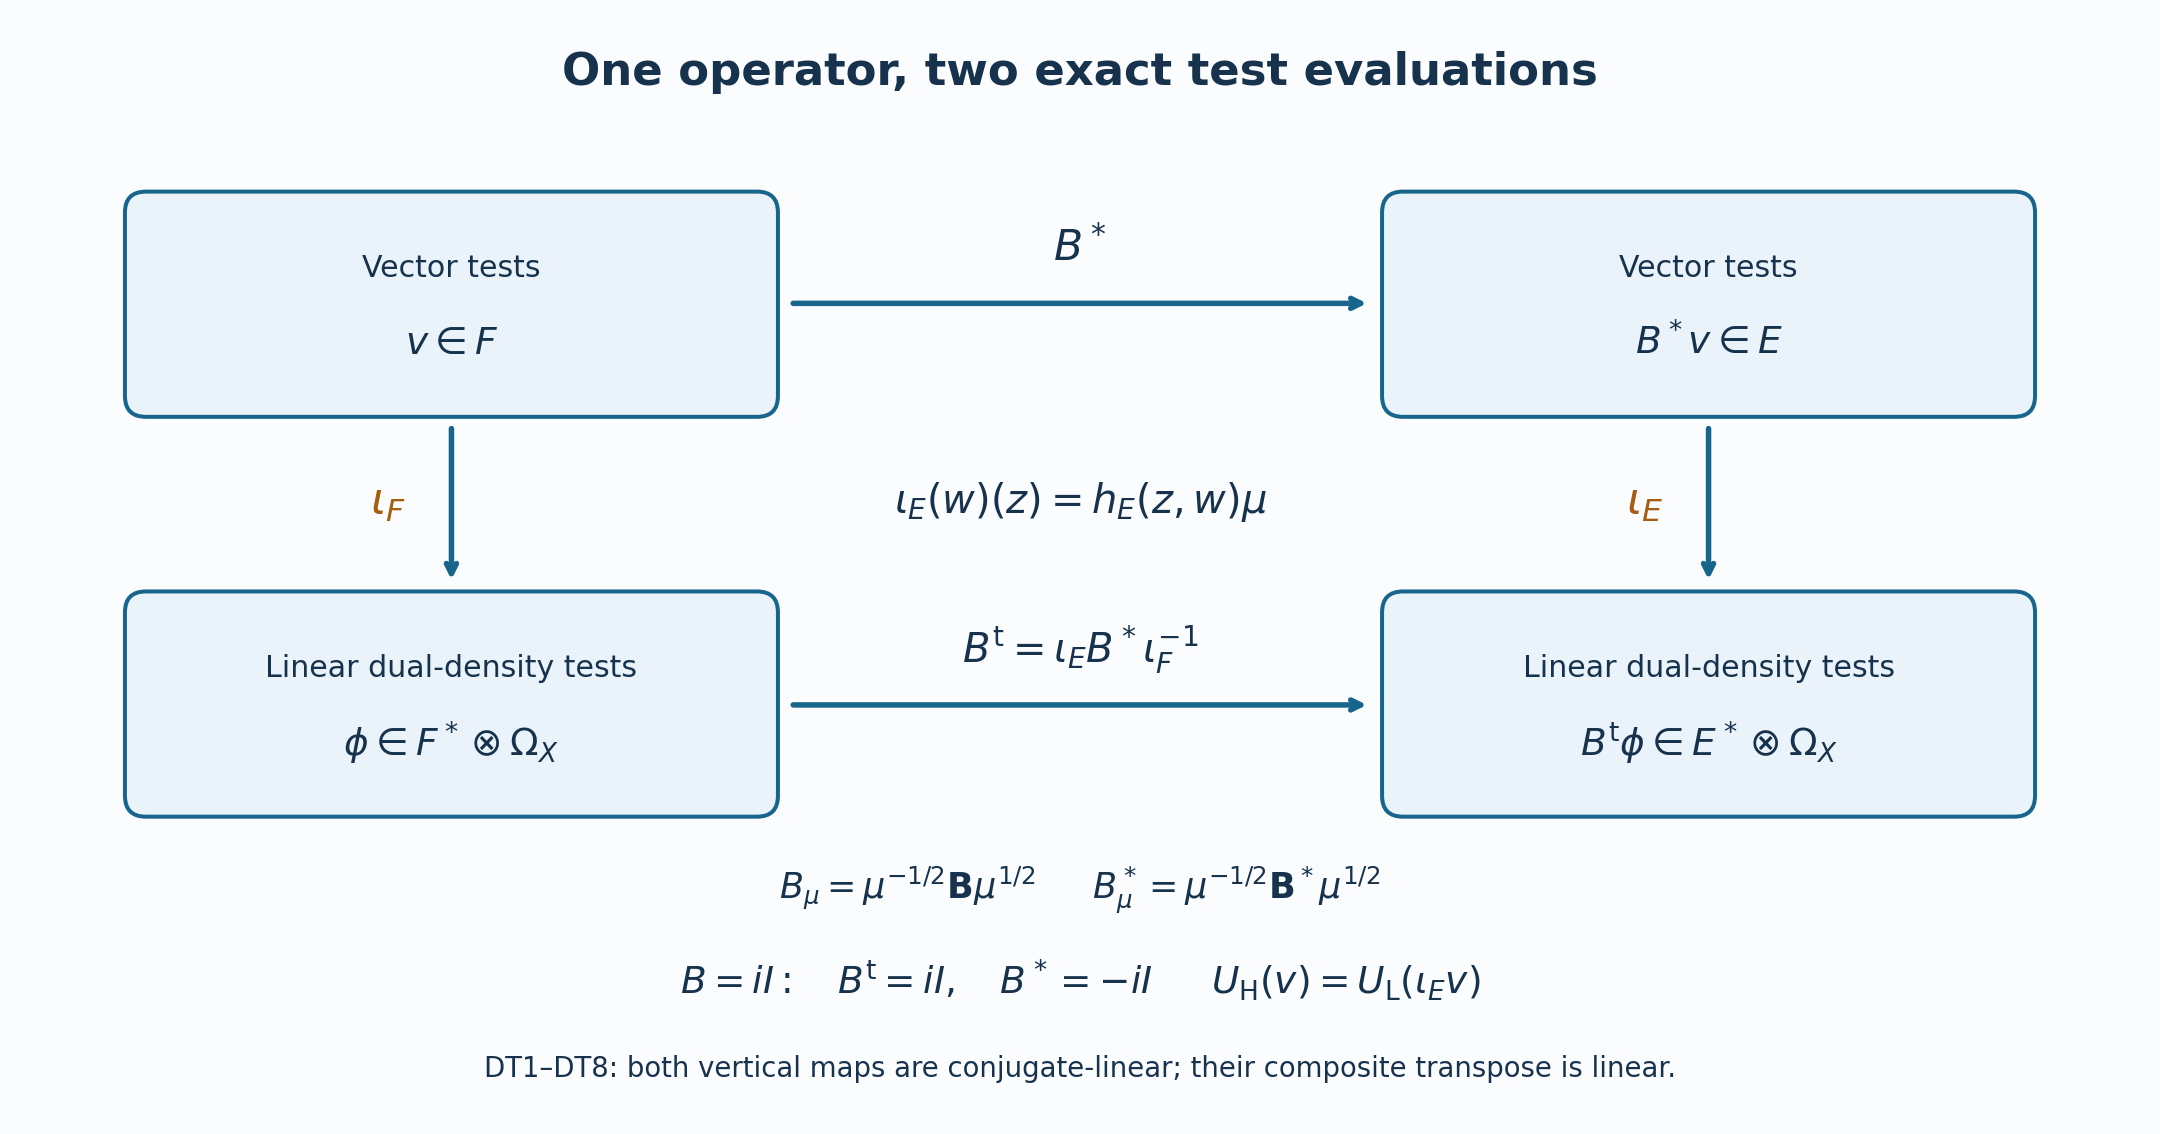
\includegraphics[keepaspectratio,alt={The exact transpose and Hermitian-adjoint maps}]{../figures/linear-and-hermitian-duals.png}}
\caption{The exact transpose and Hermitian-adjoint maps}
\end{figure}

The two arrows \(\iota_F,\iota_E\) include the complete metric and
density. Their square commutes by (DT4), and (DT5) transports the same
operator to its two dual evaluations. The half-density factors are
(DT3), and the scalar phase test is (DT8).

\ReaderArmAliases{\ReaderOriginalAnchorStart{AN03-GBD-004}\ReaderOriginalAnchorEnd\begingroup\expandafter\def\csname @currentHref\endcsname{AN03-GBD-004}\label{AN03-GBD-004}\endgroup\ReaderOriginalAnchorStart{4-compressed-wave-fronts}\ReaderOriginalAnchorEnd\begingroup\expandafter\def\csname @currentHref\endcsname{4-compressed-wave-fronts}\label{4-compressed-wave-fronts}\endgroup}
\subsection{4. Compressed wave fronts}\label{compressed-wave-fronts}

\subsubsection{4.1. Ellipticity and the characteristic set at every
symbol
order}\label{ellipticity-and-the-characteristic-set-at-every-symbol-order}

Let \(B\in\Psi_b^m(X;E,F)\) and let \(b\) be its complete local symbol.
At a nonzero compressed covector \(q=(x_0,\zeta_0)\), call \(B\)
elliptic if the two bundle ranks agree and there are a base neighborhood
\(U\), an open cone \(\Gamma\) containing \(\zeta_0\), constants
\(c,R>0\), and local frames such that \[
 b(x,\zeta):E_x\to F_x\text{ is invertible},\qquad
 \|b(x,\zeta)^{-1}\|\le c^{-1}\langle\zeta\rangle^{-m}
 \quad(x\in U,\ \zeta\in\Gamma,\ |\zeta|\ge R).
 \tag{GW1}
\] The set of covectors where this fails is \(\operatorname{Char}B\).
Changing the representative by \(S^{m-1}\) does not change (GW1):
\(b_0^{-1}(b-b_0)\) is \(O(\langle\zeta\rangle^{-1})\), so for large
\(|\zeta|\) its ordered Neumann series is invertible. Smooth frame
changes conjugate or left/right multiply by uniformly invertible
matrices on a smaller compact chart. Thus the definition is intrinsic.
The complement of the characteristic set is open and conic; the set
itself is closed and conic in \(\widetilde T^*X\setminus0\).

The inverse in (GW1) has the exact order \(-m\) on a smaller cone.
Differentiate \(b^{-1}b=I_E\): \[
 \partial_{\zeta_j}b^{-1}
   =-b^{-1}(\partial_{\zeta_j}b)b^{-1},\qquad
 \partial_{x_j}b^{-1}
   =-b^{-1}(\partial_{x_j}b)b^{-1}.
 \tag{GW2}
\] Repeated product differentiation keeps the original matrix order.
Every frequency derivative lowers the order by one; every base
derivative leaves it unchanged. Multiplying by a conic cutoff gives a
global chart symbol of order \(-m\). This proves the symbol estimate
needed for an actual microlocal parametrix.

Here is the complete construction. Choose nested cones
\(\Gamma_0\Subset\Gamma_1\Subset\Gamma\) and base neighborhoods
\(U_0\Subset U_1\Subset U\), with a smooth large-frequency cutoff
\(\chi\) supported in \(U_1\times\Gamma_1\) and equal to one on
\(U_0\times\Gamma_0\) for \(|\zeta|\) large. Set \(c_0=\chi b^{-1}\),
with the original map \(F\to E\). The lacunary realization (GC6)--(GC7)
changes this by a residual symbol only. The ordered product gives \[
 c_0\# b=\chi I_E+e_1,\qquad e_1\in S^{-1},
 \quad e_1\text{ residual away from the elliptic working cone}.
 \tag{GW3}
\] Suppose the sum \(c_0+\cdots+c_{N-1}\) has error \(e_N\in S^{-N}\),
residual away from that cone. Its next correction is \[
 c_N=-\chi_1e_N b^{-1}\in S^{-m-N},
 \qquad (e_N+c_N b)=0
 \quad\text{where }\chi_1=1\text{ on the nonresidual support of }e_N.
 \tag{GW4}
\] The actual product \(c_N\# b-c_Nb\) is one order lower by (GC9), so
the new error is in \(S^{-N-1}\), still residual off the elliptic cone.
The cutoff \(\chi_1\) is supported inside the cone where \(b^{-1}\)
exists. At each stage the part not cancelled by \(\chi_1=1\) was already
residual; include it in the final residual instead of dividing it by
\(b\). Asymptotic summation (GC13) produces a single properly supported
\(C\in\Psi_b^{-m}(F,E)\) with the global localized identity \[
 CB=Q+R,
 \qquad Q=\operatorname{Op}(\chi I_E)\in\Psi_b^0(E,E),
 \quad R\in\Psi_b^{-\infty},
 \tag{GW5}
\] and \(Q\) is elliptic on \(U_0\times\Gamma_0\). The low-frequency
part and all coordinate-patching errors are residual, and every finite
error is retained until its correction in (GW4). The same construction
on \(b c=I_F\) yields a right parametrix when needed; it is a separate
ordered calculation, not inferred by commuting the matrices in (GW4).

\subsubsection{4.2. The compressed wave-front
set}\label{the-compressed-wave-front-set}

For a supported distribution \(u\in\mathcal D'_X\), define \[
 \operatorname{WF}_b(u)
 :=\bigcap_{\substack{B\in\Psi_b^0(X;E,E)\text{ proper}\\
                         Bu\in\mathcal A(X;E)}}
       \operatorname{Char}B
 \quad\subset\widetilde T^*X\setminus0 .
 \tag{GW6}
\] The zero operator is always an admissible test, with characteristic
set equal to the whole nonzero compressed bundle. The identity is an
admissible test exactly when \(u\in\mathcal A(X)\). Thus the family of
tests is never empty. Every characteristic set is closed and conic by
(GW1), and so is its intersection. At a covector outside
\(\operatorname{WF}_b(u)\) there is one properly supported order-zero
\(B\), elliptic there, with \(Bu\in\mathcal A\). The target cannot be
changed to \(C^\infty(X)\) for arbitrary supported distributions: (GA5)
receives a residual operator into \(\mathcal A\), and its original
corner kernel may fail to smooth at the boundary.

For later use we prove the finite-cover consequence of (GW6). If
\(\operatorname{WF}_b(u)\) is empty above a compact \(K\subset X\), the
compressed unit cosphere above \(K\) has a finite cover by cones where
order-zero operators \(B_1,\ldots,B_N\) are elliptic and
\(B_ju\in\mathcal A\). Choose a smooth partition of unity \(\chi_j\) in
those cones at \(|\zeta|\ge R\), summing to a spatial cutoff
\(\varphi=1\) near \(K\). Apply (GW3)--(GW4) separately to the symbols
\(\chi_j b_j^{-1}\), preserving their factor order. Asymptotic summation
gives properly supported \(C_j\) and a residual \(R\) such that \[
 \sum_{j=1}^N C_jB_j=\varphi+R.
 \tag{GW7}
\] The missing compact-frequency part is a residual kernel and is
included in \(R\). Choose the output supports of all \(C_j\) in one
compact neighborhood of \(\operatorname{supp}\varphi\). Then \(R\) has
compact output support; proper support gives one compact input set.
Choose a compact smooth \(\psi\) equal to one on that input set. The
exact identity \(Ru=R(\psi u)\) lets (GA5) apply to the compact
distribution \(\psi u\), even when the original \(u\) is not compact.
Acting on \(u\), every \(C_j(B_ju)\) belongs to \(\mathcal A\) by (GA3),
and \(Ru\in\mathcal A\) by (GA5). Thus \(\varphi u\in\mathcal A\). On a
noncompact manifold the order obtained from this finite cover may depend
on the compact set. Retain the original class
\(\mathcal A=\bigcup_m\mathcal A^m\), and define its exact local
enlargement by

\[
 \mathcal A_{\mathrm{loc}}(X)
 =\{u\in\mathcal D'_X:
       \chi u\in\mathcal A(X)\text{ for every }\chi\in C_c^\infty(X)\}.
 \tag{GW8a}
\]

Multiplication and restriction give the injective map
\(\mathcal A\hookrightarrow\mathcal A_{\mathrm{loc}}\). The preceding
finite-cover argument proves the exact replacement for the global-order
assertion:

\[
 \operatorname{WF}_b(u)=\varnothing
       \quad\Longleftrightarrow\quad u\in\mathcal A_{\mathrm{loc}}(X).
 \tag{GW8}
\]

For the converse, at any compressed covector over \(x\), choose a
compact smooth \(\chi\) equal to one near \(x\). The multiplication
operator \(\chi I\) is properly supported, elliptic at that covector,
and maps \(u\) into the original \(\mathcal A\), by (GW8a). These
testers exclude every covector. For the forward implication, apply (GW7)
on a compact neighborhood of \(\operatorname{supp}\chi\), then multiply
its conormal output by \(\chi\). The maximum of the finitely many
conormal orders is one valid order for that compact output. If \(u\) has
compact support, choose \(\chi=1\) on its support; then \(\chi u=u\) and
(GW8) does imply \(u\in\mathcal A\). In particular the original
global-order equivalence holds on compact \(X\). No single order is
asserted after an infinite exhaustion.

The distinction is necessary. On \(X=\mathbb R_y\times[0,\infty)_t\), of
dimension two, choose nonzero \(\theta\in C_c^\infty((-1/4,1/4))\) and
form the actual locally finite supported distribution

\[
 u(y,t)=\sum_{j=1}^\infty\theta(y-j)\otimes\delta^{(j)}(t).
 \tag{GW8b}
\]

Each compact set meets only finitely many summands. The \(j\)-th summand
has normal amplitude \((i\tau)^j\theta(y-j)\) with inverse factor
\((2\pi)^{-1}\), so its conormal order is exactly \(j\), by the original
codimension-one shift \(m+(n-2)/4\) with \(n=2\). It belongs to
\(\mathcal A^j\), including all tangent derivatives. It does not belong
to \(\mathcal A^m\) when \(m<j\). To verify the last statement directly,
select a bounded interval in tangential frequency on which the squared
Fourier transform of \(\theta\) has positive integral. On the full sharp
dyadic annulus, restrict the normal frequency to
\(c_1 2^l<|\tau|<c_2 2^l\) strictly inside that annulus. Its squared
Fourier integral is bounded below by \(c_j2^{l(2j+1)}\). The (GA1) Besov
factor is \(2^{l(-m-1/2)}\), so the resulting norm is at least
\(c'_j2^{l(j-m)}\), which diverges for \(m<j\). Multiplying (GW8b) by a
compact cutoff equal to one around its \(j\)-th boundary support
isolates that summand. Thus (GW8b) lies in \(\mathcal A_{\mathrm{loc}}\)
and has empty compressed wave front, but lies in no \(\mathcal A^m\).
This proves strictness of the displayed injection. The quotient
\(\mathcal A_{\mathrm{loc}}/\mathcal A\) records precisely this failure
of one globally bounded order, with kernel of the quotient map equal to
the original \(\mathcal A\).

The stronger smoothness conclusion for \(u\in\mathcal A'\) needs the
separate local intersection theorem proved below. It is not being
inferred from conormality alone.

\subsubsection{4.3. Residual localization and elliptic
inclusion}\label{residual-localization-and-elliptic-inclusion}

Let \(A\in\Psi_b^m\) have a full symbol of order \(-\infty\) in a conic
neighborhood of a closed conic set \(\Gamma\). At each \(q\in\Gamma\)
choose an order-zero cutoff \(D_q\) elliptic at \(q\) whose
large-frequency symbol is supported in a smaller cone inside that
neighborhood. The full ordered product expansion (GC9) has every term
residual there: derivatives of the cutoff stay in the smaller cone,
derivatives of the full symbol of \(A\) have arbitrary negative order
there, and the exact far product term is residual. The
coordinate-invariant remainders (GC13) therefore give
\(D_qA\in\Psi_b^{-\infty}\), after harmless compact spatial
localization. By (GA5), \(D_qAu\in\mathcal A\). Hence \[
 \operatorname{WF}_b(Au)\cap\Gamma=\varnothing.
 \tag{GW9}
\] This proves precisely the conormal residual target; it makes no
unsupported boundary smoothness claim.

For the elliptic inclusion, let \(q\) be outside both
\(\operatorname{Char}B\) and \(\operatorname{WF}_b(Bu)\), where
\(B\in\Psi_b^m\) is proper. Select an order-zero tester \(D\) elliptic
at \(q\) with \(DBu\in\mathcal A\). The product \(DB\) has invertible
principal symbol \(d b\) near \(q\) in the original order; its inverse
is \(b^{-1}d^{-1}\). Apply (GW3)--(GW5) to \(DB\), choosing \(\chi\)
supported in the common elliptic cone and equal to one near \(q\). There
is an order-zero tester \(Q\) elliptic at \(q\) and a residual \(R\)
with the exact identity \(Q=E DB+R\). The first term is conormal by
(GA3), and the residual term by (GA5). Thus \(Qu\in\mathcal A\), giving
\[
 \operatorname{WF}_b(u)
   \subset\operatorname{WF}_b(Bu)\cup\operatorname{Char}B.
 \tag{GW10}
\] Every inverse and product has retained the bundle map order.

For a properly supported \(B\in\Psi_b^m\), the forward inclusion follows
by the complementary microlocal division. If
\(q\notin\operatorname{WF}_b(u)\), take an order-zero elliptic \(C\)
there with \(Cu\in\mathcal A\). Construct its right local parametrix
\(P_C\) as above, so \(P_CC=Q_0+R_0\), where \(R_0\) is residual and
\(Q_0\) has full symbol equal to the identity on a smaller cone about
\(q\) at high frequency. Choose \(D\) of order zero, elliptic at \(q\),
with full symbol supported inside that smaller cone. Put \(E=DBP_C\).
Since \(D\) is supported where the full symbol of \(Q_0\) is the
identity, the exact product (GC9) and its far residual give
\(DB(I-Q_0)\in\Psi_b^{-\infty}\). The product \(DBR_0\) is residual by
(GC10). Therefore \[
 DB=E C+R,
 \qquad E\in\Psi_b^m,\quad R\in\Psi_b^{-\infty}
 \tag{GW11}
\] with \(R=DB(I-Q_0)-DBR_0\). Thus \(DBu=E(Cu)+Ru\in\mathcal A\), so \[
 \operatorname{WF}_b(Bu)\subset\operatorname{WF}_b(u)
 \quad(B\in\Psi_b^m\text{ proper}).
 \tag{GW12}
\] The same inclusion holds for an arbitrary ordinary smooth
differential operator, including the unweighted normal derivative. We
prove this separately because \(D_n\) itself is not a totally
characteristic operator. For \(q\notin\operatorname{WF}_b(u)\), choose
\(C\) elliptic at \(q\) with \(Cu\in\mathcal A\). The left localized
parametrix gives \(P_CC=Q+R\), where the full symbol of \(Q\) is exactly
one on a high-frequency cone about \(q\) and \(R\) is residual. Thus \[
 Qu=P_C(Cu)-Ru\in\mathcal A.
 \tag{GW12a}
\] Choose an order-zero tester \(D\), elliptic at \(q\), with full
symbol supported in a smaller cone where \(Q=I\) microlocally. Then
\(D(I-Q)\) is residual by (GC9), including its exact far term. The
ambient supported distribution \(D_j u\) is again supported in the
closed half-space. The local commutators are exactly \[
 [D_j,T_a]=T_{D_{x_j}a}\quad(j<n),\qquad
 [D_n,T_a]=T_{D_{x_n}a}+T_{D_{\xi_n}a}D_n .
 \tag{GW12b}
\] These are the unmodified (5.1), with \(D=-i\partial\) and all signs
retained. They first hold on interior compact smooth functions. Theorem
9.1(e) in the local prerequisite approximates every supported
distribution weakly by such functions; each term in (GW12b) is a
composition of weakly continuous operators on supported distributions.
Taking that limit proves the same identity for the actual supported
representatives, including any boundary deltas.

Write \(w=(I-Q)u\). Since the full symbol of \(Q\) is constant one on
the working cone, the symbols \(D_{x_j}q\) and \(D_{\xi_n}q\) vanish
there to every symbol order. Apply \(D\) on the left in (GW12b) and use
(GC9): each resulting product is residual. The exact identity \[
 D D_jw
   =D(I-Q)D_ju+D[D_j,I-Q]u
 \tag{GW12c}
\] is therefore a sum of residual operators applied to supported
distributions, \(u\) or \(D_nu\). It belongs to \(\mathcal A\) by (GA5).
On the other hand \(Qu\in\mathcal A\) by (GW12a), and the ordinary
differential map (C17) gives \(D_jQu\in\mathcal A\); applying \(D\)
preserves that class by (GA3). Hence \(DD_ju\in\mathcal A\), so \[
 \operatorname{WF}_b(D_ju)\subset\operatorname{WF}_b(u)
 \quad(j=1,\ldots,n).
 \tag{GW12d}
\] Smooth coefficient multiplication is in \(\Psi_b^0\), and (GW12)
applies to it. Finite sums and products of the \(D_j\) with such
coefficients therefore give the same inclusion for every ordinary smooth
differential operator. The proof has kept the normal
\(T_{D_{\xi_n}a}D_n\) term in (GW12b); omitting it would make the
boundary claim unjustified.

\subsubsection{4.4. Interior comparison and a noncharacteristic
boundary}\label{interior-comparison-and-a-noncharacteristic-boundary}

In the interior, (GL8) is the ordinary cotangent identification.
Localized global \(b\)-operators are ordinary pseudodifferential
operators there by (GL13)--(GL15), and every ordinary properly supported
local operator can be realized with the same interior kernel in the
global class, using (GC7). Also \(\mathcal A\) restricts to \(C^\infty\)
in the interior by (GA1): every derivative is a combination of tangent
derivatives on a compact interior chart, and the local Sobolev estimates
give all smooth derivatives. Both implications in the tester definition
therefore give the exact equality \[
 \operatorname{WF}_b(u)|_{T^*X^\circ}
       =\operatorname{WF}(u|_{X^\circ}).
 \tag{GW13}
\]

Let \(P=\sum_{|\alpha|\le m}a_\alpha(x)D^\alpha\) be a smooth ordinary
differential operator of positive integer order \(m\), and let \(\phi\)
vanish simply at the boundary, with \(\phi=c x_n\), \(c(x',0)>0\), in a
chart. No original coefficient is removed. The complete differential
expression \[
 \phi^mP
   =\sum_{|\alpha|\le m}
      c(x)^m x_n^{m-\alpha_n}
      a_\alpha(x)D'^{\alpha'}
       \bigl(x_n^{\alpha_n}D_n^{\alpha_n}\bigr)
 \tag{GW14}
\] retains every lower-order and tangential term; the displayed factor
order is valid because \(D'\) commutes with \(x_n\). Thus
\(\phi^mP\in\operatorname{Diff}_b^m\). At \(x_n=0\), all principal terms
except \(\alpha=(0,m)\) contain a positive power of \(x_n\). Its
complete boundary principal compressed symbol is \[
 \sigma_m(\phi^mP)(x',0,\xi',\rho)
     =c(x',0)^m a_{(0,m)}(x',0)\rho^m.
 \tag{GW15}
\] If the boundary is noncharacteristic, the original leading normal
coefficient \(a_{(0,m)}(x',0)\) is invertible. Equation (GW15) is
invertible exactly when \(\rho\ne0\); its boundary characteristic set is
precisely the embedded tangential hyperplane
\(T^*\partial X=\{\rho=0\}\), with the zero section excluded. Applying
the full inclusion (GW10) to the actual operator \(\phi^mP\) yields \[
 \operatorname{WF}_b(u)|_{\partial X}
  \subset
  \operatorname{WF}_b(\phi^mPu)|_{\partial X}
        \cup(T^*\partial X\setminus0).
 \tag{GW16}
\] For \(m=0\), \(P\) is multiplication by its original invertible
coefficient under the corresponding noncharacteristic hypothesis; the
same parametrix gives (GW16) with an empty boundary characteristic set.
Formula (GW14) is not used with a negative power.

\ReaderArmAliases{\ReaderOriginalAnchorStart{AN03-GBD-005}\ReaderOriginalAnchorEnd\begingroup\expandafter\def\csname @currentHref\endcsname{AN03-GBD-005}\label{AN03-GBD-005}\endgroup\ReaderOriginalAnchorStart{5-noncharacteristic-normal-extension}\ReaderOriginalAnchorEnd\begingroup\expandafter\def\csname @currentHref\endcsname{5-noncharacteristic-normal-extension}\label{5-noncharacteristic-normal-extension}\endgroup}
\subsection{5. Noncharacteristic normal
extension}\label{noncharacteristic-normal-extension}

\subsubsection{5.1. The exact local conormal
seminorms}\label{the-exact-local-conormal-seminorms}

Fix \(K=K_0\times[0,c/2]\) compactly contained in the coordinate chart,
and use a slightly larger compact \(K'\). For \(\kappa_k=-k-n/4\), the
conormal topology on supported tests is generated by \[
 p_{k,K,L}(\phi)
 =\sum_{|\alpha|\le L}
       \|x_n^{\alpha_n}D^\alpha\phi\|_{B^{\kappa_k}_{2,\infty}}
 \quad(L=0,1,2,\ldots).
 \tag{GE1}
\] Smooth chart cutoffs are inserted in each norm. Formula (GA2) proves
that these weighted normal derivatives span exactly the same filtered
family as all words in \(D'\) and \(x_nD_n\). No lower term of the
triangular polynomial relation is dropped. Tangential differential
operators \(a(x,D')\), of \emph{any} fixed finite order, and their
formal transposes map each \(\mathcal A^k_K\) continuously into
\(\mathcal A^k_{K'}\). To verify this, expand a tangent word through
\(a\): every resulting term is another finite tangent word with smooth
coefficients, including the derivatives of those coefficients.
Multiplication by a compact smooth coefficient is bounded on each
\(B^{\kappa_k}_{2,\infty}\) by (C2)--(C3). The number of seminorms
needed depends on the actual tangential order; no relation to the normal
order is assumed.

For later use, the dyadic Fourier estimates give, for every real \(s\),
\[
 \|w\|_{B^s_{2,\infty}}
 \le C_s\left(\|w\|_{B^{s-1}_{2,\infty}}
       +\sum_{j=1}^{n}\|D_jw\|_{B^{s-1}_{2,\infty}}\right).
 \tag{GE2}
\] On the low-frequency block the first norm controls the left side. On
the \(l\)-th high block, \(2^l\asymp(\sum_j|\xi_j|^2)^{1/2}\); multiply
its \(L^2\) norm by \(2^{l(s-1)}\), use Plancherel for each \(D_j\), and
take the supremum over \(l\). This proves (GE2) without a boundary norm
convention or an omitted tangential term.

\subsubsection{5.2. The normal primitive gains one conormal
order}\label{the-normal-primitive-gains-one-conormal-order}

For \(\phi\in C_c^\infty(X^\circ)\) with support in \(K\), put \[
 \psi(x',t)=i\int_0^t\phi(x',s)\,ds,
 \qquad D_n\psi=\phi,
 \quad \psi=0\text{ below the normal support of }\phi.
 \tag{GE3}
\] Choose a fixed normal cutoff \(\chi(t)\) equal to one on \([0,c/2]\)
and supported in \([0,c)\). Then \(\chi\psi\) has compact support in the
interior for each such \(\phi\), although the distance of that support
from the boundary need not be uniform.

We first prove that the localized Volterra operator
\(J:\phi\mapsto\chi\psi\) is bounded on \(B^s_{2,\infty}\) for every
real \(s\), with fixed chart cutoffs. For this ambient-space estimate,
choose a smooth input cutoff equal to one on the original \(K\),
extending a short distance across \(t=0\), and write the integral as
\(i\chi(t)\int_{-\infty}^{t}\theta(s)\phi(x',s)\,ds\). For the original
interior-supported \(\phi\) this is exactly (GE3) after multiplication
by \(\chi\). The smooth cutoff is necessary in the negative-order dual
estimate; a sharp input cutoff at zero would create an unjustified
boundary multiplier. For \(s=0\), Cauchy--Schwarz on the finite normal
interval gives \(\|\psi\|_{L^2}\le c\|\phi\|_{L^2}\). For a nonnegative
integer \(p\), differentiate \(\chi\psi\) at most \(p\) times.
Tangential derivatives commute with the integral; each positive normal
derivative of \(\psi\) is the corresponding derivative of \(\phi\) of
one lower order; derivatives of \(\chi\) multiply the same expressions.
Thus \(J:H^p\to H^p\) is bounded. Choose these fixed cutoffs real
valued. The Hermitian adjoint has the reversed integral
\(g(s)\mapsto-i\theta(s)\int_s^c\chi(t)g(t)\,dt\). The bilinear
transpose has the full factor \(+i\); both identities and their exact
relation are proved in (DT10), Section 3.6. Its derivatives obey the
same integer estimates, including the derivatives of the smooth
\(\theta\), so duality gives \(J:H^{-p}\to H^{-p}\). For a real \(s\),
choose integers \(p<s<q\). The dyadic operator matrix estimate between
the two Sobolev endpoints is the one proved from (C2)--(C3): after
weighting by \(2^{ls-js}\), it decays geometrically in \(|l-j|\).
Summation proves the claimed \(B^s_{2,\infty}\) bound, including
negative indices. The constants depend on the fixed cutoffs, not on how
near the input support is to \(t=0\).

Now set \(s=\kappa_k=-k-n/4\). We prove the stronger precise primitive
estimate \[
 p_{k,K',L}(\chi\psi)
 \le C_{k,K,L}\,p_{k+1,K,L'}(\phi)
 \quad\text{for a finite }L'=L'(L),
 \tag{GE4}
\] since \(\kappa_{k+1}=s-1\). For a tangent word with no normal
derivative, \(D'^\beta(\chi\psi)=J(D'^\beta\phi)\), so the Volterra
bound controls its \(B^{s-1}\) norm by the corresponding \(\phi\)
seminorm. Apply (GE2) to gain the missing one degree. Its tangential
derivatives are \(J(D'^{\beta+e_j}\phi)\), and its normal derivative is
\(\chi D'^\beta\phi+(D_n\chi)D'^\beta\psi\). The same Volterra estimate
controls all these \(B^{s-1}\) norms by a finite set of (GE1) seminorms
for \(\phi\).

For a word with positive normal order \(a\ge1\), preserve its entire
normal weight: \[
 x_n^aD_n^aD'^\beta\psi
   =x_n^aD_n^{a-1}D'^\beta\phi.
 \tag{GE5}
\] The right side has a factor \(x_n\) times a tangent word in \(\phi\),
so its \(B^{s-1}\) norm is controlled. Its normal derivative is \[
 D_n(x_n^aD_n^aD'^\beta\psi)
  =x_n^aD_n^aD'^\beta\phi
      -ia\,x_n^{a-1}D_n^{a-1}D'^\beta\phi.
 \tag{GE6}
\] This is the full product rule, including its \(-ia\) term; when
\(a=0\) that term is absent and the earlier calculation applies. The
tangential derivative is \(x_n^aD_n^{a-1}D'^{\beta+e_j}\phi\), again a
smooth multiple of a tangent word. A cutoff derivative contributes
\((D_n\chi)x_n^aD_n^{a-1}D'^\beta\phi\), which has the same bound.
Applying (GE2) proves the \(B^s\) estimate for each word, and summing
finitely many words proves (GE4).

\subsubsection{5.3. First-order normal equations at every test
order}\label{first-order-normal-equations-at-every-test-order}

Let \(A_0(x,D')\) be a finite matrix of tangential differential
operators with smooth coefficients of arbitrary finite orders, and let
the extendible interior vector distribution \(u\) solve \[
 (D_n+A_0(x,D'))u=f\quad\text{in }X^\circ,
 \qquad f\in\mathcal A'(X).
 \tag{GE7}
\] We prove that \(u\) has a unique extension in \(\mathcal A'\). For
interior compact smooth tests \(\phi\) supported in \(K\), we first
establish the bound \[
 |u(\phi)|\le C_{k,K}p_{k,K,L}(\phi)
 \tag{GE8}
\] for every real \(k\), with a finite \(L\) depending on \(k,K\). Since
\(u\) is extendible, choose one ambient distribution extension
temporarily. On a fixed compact set it has finite order \(M\), so its
action on interior \(\phi\) is bounded by finitely many \(C^M\)
seminorms. Choose \(s>M+n/2\). Fourier inversion and Cauchy--Schwarz
bound those seminorms by \(H^s\), and a slightly larger
\(B^{s+\epsilon}_{2,\infty}\) norm bounds \(H^s\) by a geometric dyadic
sum. Choose \(k_0\) sufficiently negative that \(-k_0-n/4>s+\epsilon\).
The \(\alpha=0\) term of (GE1) then proves (GE8) for \(k_0\). The
extension's boundary values do not enter this interior-test estimate.

Assume (GE8) at some \(k\). Let \(\psi\) be (GE3), \(\chi\) the fixed
cutoff, and use the bilinear distribution pairing. The formal tangential
transpose \(A_0^{\mathrm t}\) retains every coefficient derivative and
reverses the matrix maps. Since \(D_n(\chi\psi)=\phi+(D_n\chi)\psi\) on
the support of \(\phi\), the exact equation (GE7) gives \[
 u(\phi)
  =-f(\chi\psi)
   +u\bigl(A_0^{\mathrm t}(\chi\psi)
              -(D_n\chi)\psi\bigr).
 \tag{GE9}
\] All arguments of \(u\) in this formula are smooth and supported in
the interior. The functional \(f\) is continuous on compact
\(\mathcal A^k\) tests for every \(k\): for \(k\ge m_0\) this is its
defining property, and for \(k<m_0\) the inclusion
\(\mathcal A^k\hookrightarrow\mathcal A^{m_0}\) is continuous. The
operator \(A_0^{\mathrm t}\) and the normal cutoff multiply
\(\mathcal A^k\) continuously by Section 5.1, regardless of the
tangential order of \(A_0\). Apply the induction hypothesis and then the
\emph{full} primitive estimate (GE4). It yields (GE8) at \(k+1\), with
finite constants and a possibly larger finite \(L\). By induction (GE8)
holds at \(k_0+j\) for every integer \(j\ge0\). For an arbitrary real
\(k\), choose \(j\) with \(k_0+j\ge k\); the continuous inclusion
\(\mathcal A^k\hookrightarrow
\mathcal A^{k_0+j}\) gives the desired bound.

Construct the supported extension rather than silently identifying it
with the temporary ambient one. For a smooth boundary test \(\phi\)
supported in \(K\), let \(\mathcal Q_\varepsilon\phi\) be (GS6); it is
smooth, supported in a fixed compact subset of the interior, and
converges to \(\phi\) in \(\mathcal A^{k_1}\) for every \(k_1>m_0\), by
(GD2) and (GS7). The bounds (GE8) make \[
 U(\phi):=\lim_{\varepsilon\downarrow0}
                   u(\mathcal Q_\varepsilon\phi)
 \tag{GE10}
\] exist: use the bound at such a \(k_1\) on differences of
approximants. The limit is independent of the particular one-sided
smoothing family because both approximations converge in the same
\(\mathcal A^{k_1}\) topology. The uniform (GS2) multiplier estimate and
(GE8), followed by the continuous inclusion from \(\mathcal A^k\) to a
larger test order, prove for every \(k\ge m_0\) a finite estimate of the
form (GD3) for \(U\). The smooth-test topology bounds those conormal
seminorms by finitely many ordinary smooth seminorms, by (GD1); thus
\(U\) is a distribution on the closed chart. The supported-distribution
duality of local Theorem 9.1(a),(c) gives its ambient supported
representative. Its interior restriction is \(u\), since
\(\mathcal Q_\varepsilon\) is an approximate identity there. By (GD4),
no second \(\mathcal A'\) extension of \(u\) exists. This proves the
first-order existence and uniqueness in the exact dual topology.

\subsubsection{5.4. Full normal order by the actual companion
system}\label{full-normal-order-by-the-actual-companion-system}

Let \(m\ge1\) and retain the original normal-monic equation \[
 P=D_n^m+\sum_{j=0}^{m-1}a_j(x,D')D_n^j,
 \qquad Pu=f\text{ in }X^\circ,
 \quad f\in\mathcal A'(X).
 \tag{GE11}
\] Each \(a_j\) is an arbitrary finite-order tangential differential
operator with smooth matrix coefficients; the orders of different
\(a_j\) are not required to be at most \(m-j\). Set \(u_j=D_n^ju\),
\(0\le j<m\). Each \(u_j\) is extendible, because an ordinary derivative
of an ambient extension remains an ambient extension of the interior
derivative. The exact first-order companion system is \[
 D_n\begin{pmatrix}u_0\\u_1\\\vdots\\u_{m-1}\end{pmatrix}
 +\begin{pmatrix}
 0&-I&0&\cdots&0\\
 0&0&-I&\cdots&0\\
 \vdots&\vdots&\vdots&\ddots&\vdots\\
 a_0&a_1&a_2&\cdots&a_{m-1}
 \end{pmatrix}
 \begin{pmatrix}u_0\\u_1\\\vdots\\u_{m-1}\end{pmatrix}
 =\begin{pmatrix}0\\0\\\vdots\\f\end{pmatrix}.
 \tag{GE12}
\] For \(m=1\) this is just (GE11), with its single matrix entry
\(a_0\); the displayed larger companion matrix is read for \(m\ge2\).
Section 5.3 applies componentwise to its actual tangential matrix,
giving a unique vector extension \(U_j\in\mathcal A'\) for every \(j\).

The corrected derivative (GD9) has the same interior restriction as
\(U_{j+1}\) for \(j<m-1\). Both belong to \(\mathcal A'\), so interior
injectivity (GD4) gives the exact equality \[
 \nabla_n^{\mathrm{int}}U_j=U_{j+1},
 \qquad D_nU_j-U_{j+1}
          =-i\,(U_j|_{x_n=0})\otimes\delta(x_n),
 \quad x_n(D_nU_j-U_{j+1})=0.
 \tag{GE13}
\] Similarly the final companion equation gives \[
 \nabla_n^{\mathrm{int}}U_{m-1}
        +\sum_{j=0}^{m-1}a_j(x,D')U_j=f,
 \quad x_n\left(D_nU_{m-1}
        +\sum_{j=0}^{m-1}a_j(x,D')U_j-f\right)=0.
 \tag{GE14}
\] The tangential operators act on \(\mathcal A'\) by (GD9), with no
normal delta correction of their own.

We keep the powers of \(x_n\) through the elimination. The full
commutator is \[
 D_n(x_n^{j+1}W)
   =x_n^{j+1}D_nW-i(j+1)x_n^jW.
 \tag{GE15}
\] Start with \(U_0=D_n^0U_0\). If \(x_n^j(U_j-D_n^jU_0)=0\), then
(GE13) implies \(x_n^{j+1}(U_{j+1}-D_nU_j)=0\), while (GE15) implies
\(x_n^{j+1}D_n(U_j-D_n^jU_0)=0\). Hence induction gives \[
 x_n^jU_j=x_n^jD_n^jU_0\qquad(0\le j<m).
 \tag{GE16}
\] Apply (GE15) once more at \(j=m-1\) to replace the first term of
(GE14) after multiplication by \(x_n^m\). For each lower term \(j<m\),
\(x_n\) commutes with \(a_j(x,D')\), and \(x_n^m a_j(U_j-D_n^jU_0)
=x_n^{m-j}a_jx_n^j(U_j-D_n^jU_0)=0\). Therefore the complete weighted
equation is \[
 x_n^m(PU_0-f)=0.
 \tag{GE17}
\] No original tangential coefficient or lower normal term was removed.

\subsubsection{5.5. Uniqueness among all supported distribution
extensions}\label{uniqueness-among-all-supported-distribution-extensions}

Let \(V\) be the difference of two supported distribution extensions of
the same interior \(u\), each satisfying (GE17). Then
\(\operatorname{supp}V\subset\{x_n=0\}\). We derive its finite normal
structure here. Localize to a compact chart and let \(M\) bound the
distribution order of \(V\). Taylor-expand a test \(h(x',t)\) through
degree \(M\) at \(t=0\), with a fixed normal cutoff \(\eta(t)=1\) near
zero: \[
 h(x',t)=\eta(t)\sum_{j=0}^{M}
       \frac{t^j}{j!}\partial_t^jh(x',0)+t^{M+1}r(x',t)
 \quad\text{near }\operatorname{supp}V.
 \tag{GE18a}
\] The remainder has every normal derivative through degree \(M\) zero
on \(t=0\); multiplication by a cutoff supported in a shrinking normal
neighborhood and the order-\(M\) bound show that \(V\) annihilates it.
Define tangential distributions \(v_j(g)=(-1)^jV(\eta(t)t^jg(x')/j!)\).
Then applying \(V\) to (GE18a) gives, with no omitted coefficient, \[
 V=\sum_{j=0}^{\mu}v_j(x')\otimes\delta^{(j)}(x_n),
 \qquad v_\mu\ne0\text{ unless }V=0.
 \tag{GE18}
\] Here \(\mu\le M\) is the highest nonzero coefficient. The definition
of \(v_j\) is independent of the cutoff because \(V\) is supported at
\(t=0\). The local representations agree on overlapping charts, so this
argument applies to every compactly supported piece of \(V\). The
coefficients are tangential distributions, possibly vector valued. The
normal distribution formulas, with every factor, are \[
 D_n^k\delta^{(j)}=(-i)^k\delta^{(j+k)},\qquad
 x_n^m\delta^{(j+k)}
 =\begin{cases}
 (-1)^m\dfrac{(j+k)!}{(j+k-m)!}\delta^{(j+k-m)},&j+k\ge m,\\
 0,&j+k<m.
 \end{cases}
 \tag{GE19}
\] They follow by applying the distributions to a test function and
differentiating \(x_n^m\) exactly \(m\) times at zero; no coefficient is
normalized away. In \(x_n^mPV\), the original leading term
\(x_n^mD_n^m(v_\mu\delta^{(\mu)})\) has the top normal coefficient \[
 i^m\frac{(\mu+m)!}{\mu!}
       v_\mu(x')\otimes\delta^{(\mu)}(x_n),
 \tag{GE20}
\] which is nonzero when \(v_\mu\ne0\). Every lower normal term
\(a_j(x,D')D_n^j\), \(j<m\), has normal order at most
\(\mu+j-m\le\mu-1\) after multiplication by \(x_n^m\). Taylor
coefficients of \(a_j\) at the boundary can lower that order further,
never raise it. Contributions from \(v_l\) with \(l<\mu\) also have
order below \(\mu\). The coefficient of \(\delta^{(\mu)}\) in
\(x_n^mPV=0\) therefore forces \(v_\mu=0\), a contradiction. Repeating
downward gives \(V=0\). This proves uniqueness among \emph{all}
supported distribution extensions satisfying (GE17), stronger than
uniqueness only in \(\mathcal A'\).

The theorem so far is local on the stated product collar. The
globalization and boundary wave-front consequence are proved next.

\subsubsection{5.6. The noncharacteristic boundary wave-front
class}\label{the-noncharacteristic-boundary-wave-front-class}

Write \(\widetilde T^*X\) for the compressed cotangent bundle of
(GL11)--(GL18), and embed \(T^*\partial X\setminus0\) as its boundary
covectors with zero normal compressed component. Define the exact class
\[
 \mathcal N(X)
  :=\{v\in\mathcal A'(X):
       \operatorname{WF}_b(v)|_{\partial X}
       \subset T^*\partial X\setminus0\}.
 \tag{GE21}
\] This is a condition on the already-defined wave-front set (GW6), not
a replacement for the dual conormal requirement.

Let \(P\) be a smooth ordinary differential operator of normal order
\(m\ge1\) whose boundary is noncharacteristic, and let an extendible
interior distribution \(u\) solve \(Pu=f\) with \(f\in\mathcal N(X)\).
In one product chart retain the complete normal expansion \[
 P=a_m(x)D_n^m+
       \sum_{j=0}^{m-1}a_j(x,D')D_n^j,
 \qquad a_m(x',0)\text{ invertible}.
 \tag{GE22}
\] Shrinking the chart makes \(a_m(x)\) invertible throughout it.
Multiplying the equation on the \emph{left} by its inverse gives the
normal-monic operator \(P'=a_m^{-1}P\) and source \(f'=a_m^{-1}f\). The
order of matrix multiplication is retained. Smooth multiplication
preserves \(\mathcal A'\) by (GD13) and preserves the boundary
wave-front condition by (GW12); thus \(f'\in\mathcal N\). Sections
5.3--5.5 give the unique local \(U\in\mathcal A'\) with \[
 x_n^m(P'U-f')=0,
 \qquad x_n^m(PU-f)=0.
 \tag{GE23}
\] The second equality follows by multiplying the first on the left by
\(a_m\), which commutes with the scalar \(x_n^m\). In (GE23) the
composition \(x_n^mP\) is also its actual totally characteristic
differential action on supported distributions: the original
coefficients, their product order, and the raw ambient normal
derivatives agree with (GD13) after transposition.

The full noncharacteristic estimate (GW16), with the original defining
function \(\phi=x_n\) in this chart, applies to this \(U\): \[
 \operatorname{WF}_b(U)|_{\partial X}
 \subset
 \operatorname{WF}_b(x_n^mPU)|_{\partial X}
       \cup(T^*\partial X\setminus0)
 =\operatorname{WF}_b(x_n^mf)|_{\partial X}
       \cup(T^*\partial X\setminus0).
 \tag{GE24}
\] Multiplication by \(x_n^m\) is a proper order-zero totally
characteristic operator after localization. The full forward inclusion
(GW12), rather than an unsupported assertion about its zero set, gives
\[
 \operatorname{WF}_b(x_n^mf)|_{\partial X}
       \subset\operatorname{WF}_b(f)|_{\partial X}
       \subset T^*\partial X\setminus0.
 \tag{GE25}
\] Equations (GE24)--(GE25) prove \(U\in\mathcal N\). On overlapping
boundary charts, two such local extensions have the same interior
restriction and belong to \(\mathcal A'\), so (GD4) makes them equal.
The product coordinate changes and bundle maps preserve \(\mathcal A'\)
by (GA4) and the compressed wave-front condition by (GL11)--(GL18) and
(GW6). The local extensions therefore glue to a global
\(U\in\mathcal N(X)\), uniquely determined by the interior \(u\): \[
 Pu=f\text{ in }X^\circ,\quad f\in\mathcal N(X),\quad
 \partial X\text{ noncharacteristic for }P
 \quad\Longrightarrow\quad
 \exists!\,U\in\mathcal N(X),\ U|_{X^\circ}=u.
 \tag{GE26}
\] The uniqueness in (GE26) is also immediate from (GD4). Its existence
uses the actual weighted equation (GE23); an arbitrary ambient extension
would not supply the conclusion. For an order-zero \(P=a_0(x)\)
invertible at the boundary, local inversion gives
\(U=a_0^{-1}f\in\mathcal N\) by (GD13) and (GW12), with the same
interior restriction and uniqueness by (GD4). Thus (GE26) also covers
this endpoint without applying the positive-order companion construction
to a zero-dimensional system.

\ReaderArmAliases{\ReaderOriginalAnchorStart{AN03-GBD-006}\ReaderOriginalAnchorEnd\begingroup\expandafter\def\csname @currentHref\endcsname{AN03-GBD-006}\label{AN03-GBD-006}\endgroup\ReaderOriginalAnchorStart{6-tangential-action-at-the-boundary}\ReaderOriginalAnchorEnd\begingroup\expandafter\def\csname @currentHref\endcsname{6-tangential-action-at-the-boundary}\label{6-tangential-action-at-the-boundary}\endgroup}
\subsection{6. Tangential action at the
boundary}\label{tangential-action-at-the-boundary}

\subsubsection{6.1. The actual tangential action and the conormal
topology}\label{the-actual-tangential-action-and-the-conormal-topology}

Let \(b(x',t,\xi')\in S^d\), \(d\in\mathbb R\), smooth down to \(t=0\),
with its original full family of tangential symbol seminorms. Its left
quantization, with the same Fourier convention as (GL13), is \[
 (B_bv)(x',t)=(2\pi)^{-(n-1)}
     \int e^{i(x'-y')\cdot\xi'}b(x',t,\xi')v(y',t)
                  \,dy'\,d\xi'.
 \tag{GT1}
\] For \(n=1\), the tangential dimension is zero and (GT1) is smooth
multiplication. Insert the actual proper-support kernel cutoff of
\(B_b\) in (GT1) when needed. It maps compact smooth tests to compact
smooth tests, including in the normal variable. Its transpose
\(B_b^{\mathrm t}\) is another properly supported tangential operator of
order \(d\), with smooth \(t\)-dependent coefficients; this follows
directly by transposing the kernel and Taylor-expanding \(b(y',t,\xi')\)
in \(y'-x'\), retaining the exact far kernel as a tangential smoothing
term. Thus (GT1) acts by transposition on every distribution for which
proper support is specified, before any wave-front restriction is
imposed.

We prove the stronger topology statement needed below. With the actual
\(\mathcal A^k\) seminorms (GE1), for each compact chart \(K\), real
\(k\), and finite \(L\), there are a compact \(K'\), finite \(L'\), and
\(C\) such that \[
 p_{k,K,L}(B_bv)\le C p_{k,K',L'}(v)
 \quad(v\in\mathcal A^k_{K'}),
 \qquad
 p_{k,K,L}(B_b^{\mathrm t}v)\le C p_{k,K',L'}(v).
 \tag{GT2}
\] Here the compact sets are chosen to include the source and target of
the properly supported localized kernel. To prove the Besov part, first
localize both base variables to compact sets and extend the resulting
smooth \(x=(x',t)\)-dependence periodically on a larger box. At \(t=0\),
use the smooth collar extension of Section 3 of the linked local lesson
before periodic extension; for each finite estimate its extension bounds
involve only a finite number of the original one-sided symbol seminorms.
Its Fourier series is \[
 b(x,\xi')=\sum_{\ell\in\mathbb Z^n}
       e^{i\ell\cdot x}b_\ell(\xi'),\qquad
 |\partial_{\xi'}^\beta b_\ell(\xi')|
   \le C_{N\beta}\langle\ell\rangle^{-N}
                         \langle\xi'\rangle^{d-|\beta|}
 \quad(\forall N).
 \tag{GT3}
\] This follows by integrating by parts \(N\) times in the compact base
Fourier coefficient; every base derivative of the original symbol has
the same order \(d\). Choose an even integer \(M=2r\ge\max(d,0)\). The
full Fourier multiplier \(b_\ell(\xi')\langle\xi'\rangle^{-M}\) is
bounded uniformly in \((\xi',\xi_n)\) by \(C_N\langle\ell\rangle^{-N}\),
so it is bounded on \(B^s_{2,\infty}(\mathbb R^n)\) for every real
\(s\): it commutes with each full dyadic projection and Plancherel gives
the bound on each block. The factor
\(\langle\xi'\rangle^M=(1+|\xi'|^2)^r\) is the \emph{complete} finite
polynomial in tangential derivatives, not an isotropic replacement.
Multiplication by \(e^{i\ell\cdot x}\) shifts full frequency by
\(\ell\); direct dyadic overlap shows its \(B^s_{2,\infty}\) operator
bound grows by at most a fixed polynomial in \(\langle\ell\rangle\).
Choosing \(N\) larger than that degree plus \(n+1\), then summing (GT3),
proves \[
 \|B_bv\|_{B^s_{2,\infty}}
 \le C_{s,b}\sum_{|\beta|\le M}
          \|D'^\beta v\|_{B^s_{2,\infty}}.
 \tag{GT4}
\] The same argument applies to every normal and tangential base
derivative of \(b\), including the transpose symbol and its exact far
smoothing kernel. Its properly supported kernel cutoffs are smooth
multiplication on the two sides and obey the same estimates.

The normal variable is unchanged by the kernel in (GT1), hence
\(t^aB_b=B_bt^a\). Differentiate the full expression rather than
identifying normal and tangential orders: \[
 t^aD_n^aD'^\gamma(B_bv)
 =\sum_{j=0}^{a}\sum_{\beta\le\gamma}
       \binom aj\binom\gamma\beta
       t^j B_{D_n^jD_{x'}^\beta b}
        \bigl(t^{a-j}D_n^{a-j}D'^{\gamma-\beta}v\bigr).
 \tag{GT5}
\] The formula also applies termwise to the proper kernel cutoff; its
derivatives are included in the differentiated symbol. Every \(t^j\) is
a smooth compact multiplier, and (GT4) controls the remaining tangential
operator by finitely many further \(D'\) seminorms. This proves (GT2),
with \emph{each} original normal weight and derivative retained. In
particular \(B_b\) and \(B_b^{\mathrm t}\) preserve every filtered
\(\mathcal A^k\), and the dual formula \[
 (B_bu)(v)=u(B_b^{\mathrm t}v)
 \tag{GT6}
\] defines a weakly continuous map \(\mathcal A'\to\mathcal A'\). The
stronger action statement follows from the explicit topology estimate;
it does not identify \(B_b\) with an isotropic \(n\)-covariable
pseudodifferential symbol.

\subsubsection{6.2. The equatorial compressed
cutoff}\label{the-equatorial-compressed-cutoff}

Choose a smooth conic symbol \(t_0(\xi',\rho)\) of order zero,
independent of \(x'\), with the original low-frequency cutoff, so that
\[
 t_0=1\quad(2|\rho|<|\xi'|,\ |\xi'|>1),\qquad
 t_0=0\quad(|\rho|>|\xi'|).
 \tag{GT7}
\] Multiply by a smooth normal base cutoff equal to one on \(0\le t<1\)
and supported in \(t<2\). The construction on the unit sphere is
possible because the closed equatorial band and the normal caps are
disjoint. Apply the \emph{original} lacunarization of Lemma 4.4 to this
full symbol and write \(t_\rho\in S^0_{\mathrm{la}}\). The difference
\(t_\rho-t_0\) is residual, with its original normal-base decay; it does
not change the principal compressed symbol. Let \(T=T_{t_\rho}\),
localized properly in a boundary chart.

For \(u\in\mathcal N\), put \(w=(I-T)u\). At every boundary tangential
covector \(q\), the full symbol of \(I-T\) vanishes on a conic
neighborhood of \(q\), so (GW9) removes \(q\) from
\(\operatorname{WF}_b(w)\). At every other boundary covector \(q\), the
definition of \(\mathcal N\) removes \(q\) from
\(\operatorname{WF}_b(u)\), and (GW12) removes it from
\(\operatorname{WF}_b(w)\). Thus the boundary portion is empty: \[
 \operatorname{WF}_b((I-T)u)|_{\partial X}=\varnothing.
 \tag{GT8}
\] On a compact boundary patch, closedness of \(\operatorname{WF}_b\) on
the compact cosphere gives a collar in which it remains empty. The
finite microlocal cover argument (GW7) then makes a spatially localized
\(w\) an element of \(\mathcal A\). Equation (GT2) gives
\(B_bw\in\mathcal A\). We have therefore proved, as a local
\emph{conormal equality} rather than an unproved smoothness claim, \[
 B_bu=B_bTu+v,
 \qquad v\in\mathcal A\text{ near the boundary}.
 \tag{GT9}
\] The equality is between the actual distributional actions (GT6).

Because \(t_\rho\) is independent of \(x'\), the unlocalized
Kohn--Nirenberg composition in (GT1) is exact: \[
 B_bT_{t_\rho}=T_a,
 \qquad a(x',t,\xi',\rho)=b(x',t,\xi')t_\rho(t,\xi',\rho).
 \tag{GT10}
\] Indeed integration in the intermediate tangential variable gives
\((2\pi)^{n-1}\delta(\eta'-\xi')\); no derivative of \(t_\rho\) in
\(x'\) appears. The support of \(t_0\) in (GT7) ensures that on the
high-frequency nonresidual part
\(\langle\xi'\rangle\asymp\langle(\xi',\rho)\rangle\). All \(\xi'\),
\(\rho\), and base derivatives of the product therefore obey the full
order-\(d\) symbol bounds. The residual difference from lacunarization
remains residual after multiplication by \(b\), using arbitrary residual
order to absorb its fixed order \(d\). Since normal Fourier convolution
does not change a tangential multiplier, the product retains the
original lacunarity. Thus \(a\in S^d_{\mathrm{la}}\).

Proper-support cutoffs make (GT10) an equality modulo a residual
\emph{full} compressed operator. To verify the asserted residual class,
write each far tangential cutoff as a kernel factor vanishing near
\(x'=y'\) and integrate by parts in \(\xi'\) arbitrarily many times. On
the nonresidual support of \(t_0\), the entire normal frequency is
bounded by a constant times \(|\xi'|\), so this gain is arbitrary in the
full \((\xi',\rho)\) order. The lacunarization remainder is already
residual. Derivatives of the cutoff and amplitude obey the same bounds,
proving the full residual assertion. Its action on supported
distributions lies in \(\mathcal A\) by (GA5), so it does not affect the
boundary wave-front conclusions.

\subsubsection{6.3. Boundary action, microsupport, and elliptic
comparison}\label{boundary-action-microsupport-and-elliptic-comparison}

The local boundary wave-front set of \(v\in\mathcal A\) is empty by
definition, and adding such a \(v\) does not change a wave-front set: a
regularizing tester for one summand works for the sum, and subtracting
the same \(v\) gives the reverse inclusion. Equations (GT9)--(GT10) and
(GW12) therefore give \[
 \operatorname{WF}_b(B_bu)|_{\partial X}
   =\operatorname{WF}_b(T_au)|_{\partial X}
   \subset\operatorname{WF}_b(u)|_{\partial X}
   \subset T^*\partial X\setminus0.
 \tag{GT11}
\] Since (GT6) also gives \(B_bu\in\mathcal A'\), this proves
\(B_b:\mathcal N\to\mathcal N\) with the original tangential operator.
It also proves that the action is continuous in the weak topology of
\(\mathcal A'\) tested on fixed conormal functions.

Suppose \(b\) is of order \(-\infty\) on a conic neighborhood of the
complement of a closed tangential cone \(\Gamma\) at the boundary. At a
tangential covector \(q\notin\Gamma\), the full symbol \(a=b t_\rho\) is
of order \(-\infty\) on a compressed cone about \(q\). The original
residual localization (GW9) excludes \(q\) from
\(\operatorname{WF}_b(T_au)\). At normal compressed directions (GT11)
already excludes every covector. Hence the exact boundary microsupport
statement is \[
 \operatorname{WF}_b(B_bu)|_{\partial X}
 \subset\operatorname{WF}_b(u)|_{\partial X}\cap\Gamma.
 \tag{GT12}
\]

Write \(b_0(x',\xi')=b(x',0,\xi')\). At a tangential boundary covector
\(q=(x',0,\eta',0)\), (GT7), (GL18), and (GC4) give the actual principal
compressed symbol of \(T_a\): \[
 \sigma_d(T_a)(q)=\sigma_d(b_0)(x',\eta')\cdot 1.
 \tag{GT13}
\] The boundary operator action (GL24) has the same principal symbol,
with the original \((2\pi)^{-(n-1)}\) Fourier factor. If \(b_0\) is
elliptic at \(q\), then \(T_a\) is elliptic there. The exact elliptic
inclusion (GW10), applied to \(T_au=B_bu-v\) from (GT9), gives \[
 \operatorname{WF}_b(u)|_{\partial X}
   \subset
   \operatorname{WF}_b(B_bu)|_{\partial X}
       \cup\operatorname{Char}(b_0).
 \tag{GT14}
\] The factor order in (GT13) stays matrix order; for vector bundles,
ellipticity means the actual boundary matrix is invertible.

\subsubsection{6.4. What the argument gives in the
interior}\label{what-the-argument-gives-in-the-interior}

At an interior point \((x',t)\), \(t>0\), the tangential action is the
family (GT1). The full kernel is a tangential pseudodifferential kernel
times \(\delta(t-s)\). Split it with a cutoff in \(x'-y'\) that is one
near zero. Off the tangential diagonal the tangential kernel is smooth,
by arbitrary integration by parts in \(\xi'\). Its output can therefore
be singular only in the normal variable, so every covector there has
\(\xi'=0\). On the tangential diagonal, fix an output covector with
\(\xi'\ne0\) and take a conic cutoff on which
\(|\xi'|\ge c|(\xi',\xi_n)|\) for some \(c>0\). The full symbol
\(b(x,\xi')\) obeys the ordinary isotropic symbol estimates on that
cone, since its only frequency derivatives are in \(\xi'\) and
\(\langle\xi'\rangle\asymp\langle\xi\rangle\) there. The complementary
frequency cutoff has no output wave-front in this cone by nonstationary
integration in the full oscillatory kernel. The standard local
integration-by-parts proof of pseudolocality therefore applies to the
retained kernel. Together with (GW13), this gives the exact interior
inclusion \[
 \operatorname{WF}_b(B_bu)|_{T^*X^\circ\cap\{\xi'\ne0\}}
       \subset
       \operatorname{WF}_b(u)|_{T^*X^\circ\cap\{\xi'\ne0\}}.
 \tag{GT15}
\] The region on which (GT15) is useful depends on the actual wave-front
covectors of \(u\). It does not claim an all-interior inclusion: at
\(\xi'=0\), a tangential smoothing kernel can carry a normal singularity
between distinct tangential points at the same \(t\), precisely because
the kernel still contains \(\delta(t-s)\). For example, take a properly
supported smooth tangential kernel \(K(x',y')\) with
\(K(x'_1,y'_0)\ne0\) and \(x'_1\ne y'_0\), and
\(u=\delta(x'-y'_0)\otimes\delta(t-t_0)\) with \(t_0>0\). Then
\(B_bu=K(x',y'_0)\delta(t-t_0)\) has a pure-normal wave-front covector
at \((x'_1,t_0)\), while \(u\) has no wave-front there. This proves that
the exception is necessary, rather than leaving an all-interior claim
untested.

\ReaderArmAliases{\ReaderOriginalAnchorStart{AN03-GBD-007}\ReaderOriginalAnchorEnd\begingroup\expandafter\def\csname @currentHref\endcsname{AN03-GBD-007}\label{AN03-GBD-007}\endgroup\ReaderOriginalAnchorStart{7-the-hardy-weight-and-a-singular-test}\ReaderOriginalAnchorEnd\begingroup\expandafter\def\csname @currentHref\endcsname{7-the-hardy-weight-and-a-singular-test}\label{7-the-hardy-weight-and-a-singular-test}\endgroup}
\subsection{7. The Hardy weight and a singular
test}\label{the-hardy-weight-and-a-singular-test}

\subsubsection{7.1. The weighted norm with its complete order
shift}\label{the-weighted-norm-with-its-complete-order-shift}

Localize in a compact boundary product chart. An element
\(u\in\mathcal A^m\) has, modulo a smooth term, the exact normal
conormal oscillatory representation \[
 u(x',t)=(2\pi)^{-1}\int_{\mathbb R}
         e^{it\tau}a(x',\tau)\,d\tau,
 \qquad
 |D_{x'}^\beta\partial_\tau^j a(x',\tau)|
     \le C_{\beta j}\langle\tau\rangle^{\mu-j},
 \quad \mu=m+\frac{n-2}{4}.
 \tag{HS1}
\] This is the \emph{original} codimension-one shift, including the
ambient dimension. The inverse coefficient and \(D=-i\partial\)
convention are retained. For a normal derivative of order \(a\ge0\), the
amplitude is \(\tau^aD_{x'}^\beta a\), of order \(\mu+a\). Split its
integral at \(|\tau|=t^{-1}\), \(0<t<1\). The low-frequency absolute
integral is bounded by \(Ct^{-\mu-a-1}\) when \(\mu+a>-1\), by
\(C(1+|\log t|)\) at equality, and by \(C\) below it. On the
high-frequency part integrate by parts in \(\tau\) \(N>\mu+a+1\) times,
including the derivatives of a smooth cutoff at \(|\tau|=t^{-1}\). Each
resulting term is bounded by \(Ct^{-\mu-a-1}\). The same estimate holds
for every tangential derivative, uniformly on a smaller compact chart.
Thus the complete safe weighted \(L^2\) implication is \[
 \int_{K_0}\int_0^c
     t^{2\nu}|D'^\beta D_n^a u(x',t)|^2
                       \,dt\,dx'<\infty
 \quad\text{whenever }
 \nu\ge0,\quad \nu>m+\frac n4+a.
 \tag{HS2}
\] The strict endpoint includes the logarithmic case. Equation (HS2)
states the weight \emph{inside the norm} as \(t^\nu\); the power inside
the squared integral is \(2\nu\). A cached target record that writes a
single exponent \(N\) on the squared integral cannot be substituted for
the original formula without checking whether its \(N\) names \(\nu\) or
\(2\nu\). This is a routing ambiguity, not a claim of an error in a
human source.

\subsubsection{7.2. Hardy's exact coefficient and the failed direct
iteration}\label{hardys-exact-coefficient-and-the-failed-direct-iteration}

Let \(v\in C_c^\infty((0,\infty))\) and \(\lambda\ge0\). The boundary
terms in integration by parts vanish at both ends. Writing
\(I=\int t^{2\lambda}|v|^2dt\), \(J=\int t^{2\lambda+2}|v'|^2dt\), the
\emph{full} calculation is \[
 \begin{aligned}
 (2\lambda+1)I
  &=-\int_0^\infty t^{2\lambda+1}
                     \partial_t|v|^2\,dt\\
  &=-2\operatorname{Re}\int_0^\infty
            t^{2\lambda+1}v'\overline v\,dt
   \le2\sqrt{IJ},\\
 I&\le\frac{4}{(2\lambda+1)^2}J.
 \end{aligned}
 \tag{HS3}
\] The sign in the middle line is retained, and the last inequality uses
Cauchy--Schwarz. For a compactly supported \(v\) away from zero,
iteration at \(\lambda=0,1,\ldots,k-1\) gives \[
 \int|v|^2dt
 \le\left[\prod_{j=0}^{k-1}
          \frac{4}{(2j+1)^2}\right]
       \int t^{2k}|v^{(k)}|^2dt.
 \tag{HS4}
\] One cannot remove the cutoff at zero unless all cutoff-error terms
and the final weighted integral have actual bounds. For
\(v=D'^\beta D_n^a u\), using only (HS2) on the final integral would
require \[
 k>m+\frac n4+(a+k),
 \quad\text{equivalently}\quad 0>m+\frac n4+a.
 \tag{HS5}
\] When that last number is nonnegative, no choice of the number of
Hardy iterations fixes the estimate. This is the exact remaining deficit
of the \emph{conormal-only} argument, including both the original order
and the derivative count. It identifies where \(u\in\mathcal A'\) must
enter; it is not a proof of \(\mathcal A'\cap\mathcal A=C^\infty\).

\subsubsection{7.3. A singular conormal test of the missing
hypothesis}\label{a-singular-conormal-test-of-the-missing-hypothesis}

In one normal dimension choose \(\chi\in C_c^\infty([0,\infty))\) equal
to one near zero and put \(u(t)=\chi(t)t^{-3/4}H(t)\). The Fourier
amplitude has normal order \(-1/4\), so (HS1) gives its exact conormal
order \(m=0\) when \(n=1\). It is locally integrable but not in \(L^2\),
since \(\int_0^c t^{-3/2}dt=\infty\). Moreover \(t^kD_n^ku\) has the
same leading power for every \(k\), so the final integral in (HS4)
diverges for every \(k\), exactly as (HS5) predicts.

Take a nonnegative \(q\in C_c^\infty((1,2))\) with integral one and set
\(q_\varepsilon(t)=\varepsilon^{-1}q(t/\varepsilon)\). The boundary
delta is conormal of order \((2-n)/4=1/4\) by (GD7), and (GS7) makes
\(q_\varepsilon=Q_\varepsilon\delta\) converge to \(\delta\) in every
\(\mathcal A^{m'}\) with \(m'>1/4\). Yet the ordinary interior pairing
is \[
 u(q_\varepsilon)
   =\varepsilon^{-3/4}
       \int_1^2s^{-3/4}q(s)\,ds
   \longrightarrow+\infty.
 \tag{HS6}
\] If this \(u\) belonged to \(\mathcal A'\), continuity on that
\(\mathcal A^{m'}\) would make the same pairings converge to the finite
value \(u(\delta)\). Thus \(u\in\mathcal A^0\setminus\mathcal A'\). This
example proves that the dual requirement excludes at least the displayed
power singularity; it does not replace a proof for every conormal
amplitude.

\ReaderArmAliases{\ReaderOriginalAnchorStart{AN03-GBD-008}\ReaderOriginalAnchorEnd\begingroup\expandafter\def\csname @currentHref\endcsname{AN03-GBD-008}\label{AN03-GBD-008}\endgroup\ReaderOriginalAnchorStart{8-smoothness-from-the-dual-conormal-condition}\ReaderOriginalAnchorEnd\begingroup\expandafter\def\csname @currentHref\endcsname{8-smoothness-from-the-dual-conormal-condition}\label{8-smoothness-from-the-dual-conormal-condition}\endgroup}
\subsection{8. Smoothness from the dual conormal
condition}\label{smoothness-from-the-dual-conormal-condition}

\subsubsection{8.1. Every boundary delta jet and its precise conormal
order}\label{every-boundary-delta-jet-and-its-precise-conormal-order}

For a compact smooth tangential density \(h(x')\), the normal delta
derivative has the original Fourier representation \[
 h(x')\otimes\delta^{(j)}(t)
  =(2\pi)^{-1}\int e^{it\tau}(i\tau)^j h(x')\,d\tau,
 \qquad
 m_j=\frac{2-n}{4}+j=\frac12-\frac n4+j.
 \tag{SP1}
\] The exponent \(m_j\) follows from the \emph{unmodified}
codimension-one order relation in (C16): the amplitude has order
\(j=m_j+(n-2)/4\). The factor \((2\pi)^{-1}\) and \(i^j\) have not been
absorbed. Formula (GA1) gives the same order by dyadic estimation,
including every tangent derivative. For \(u\in\mathcal A'\) define
\(g_j=(\nabla_n^{\mathrm{int},j}u)|_{t=0}\) by (GD8)--(GD9). These are
tangential distributions at this stage. For a smooth boundary \(u\),
direct differentiation and the distributional delta sign give \[
 u(h\otimes\delta^{(j)})=(-1)^j
       \langle\partial_t^ju|_{t=0},h\rangle
       =(-i)^j\langle g_j,h\rangle.
 \tag{SP2}
\] Both sides are weakly continuous on \(\mathcal A'\): the left is one
of its defining conormal-test pairings by (SP1), and the right is a
composition of the weakly continuous corrected derivative and trace maps
(GD8)--(GD9). Smooth functions are weakly dense by (GD5), so (SP2) holds
for \emph{every} \(u\in\mathcal A'\), with no assertion that the ambient
uncorrected derivative has the same trace.

\subsubsection{8.2. Quantitative scaled test expansion in the actual
topology}\label{quantitative-scaled-test-expansion-in-the-actual-topology}

Fix \(J=[1,2]\) and a compact tangential chart set. For
\(\psi\in C_c^\infty(X_0\times(1,2))\), put \[
 v_\varepsilon(x',t)=\varepsilon^{-1}
                 \psi(x',t/\varepsilon),\qquad
 M_j(x')=\int_1^2s^j\psi(x',s)\,ds.
 \tag{SP3}
\] The test is smooth and supported in the interior for each
\(\varepsilon>0\). Taylor's formula at the \emph{actual} boundary gives
the distributional expansion \[
 v_\varepsilon
  =\sum_{j=0}^{N-1}
      \frac{(-1)^j\varepsilon^j}{j!}
          M_j(x')\otimes\delta^{(j)}(t)
       +R_{N,\varepsilon}.
 \tag{SP4}
\] We need its quantitative conormal topology, not only distributional
convergence. For every integer \(N\ge1\), real \(M>m_0+N\) with
\(m_0=(2-n)/4\), compact output set \(K\), and finite tangent seminorm
index \(L\), there are finite \(L'\), \(C\) such that \[
 p_{M,K,L}(R_{N,\varepsilon})
       \le C\varepsilon^N
             \sum_{|\gamma|\le L'}
                   \|D_{x',s}^\gamma\psi\|_{L^\infty},
       \qquad0<\varepsilon\le1.
 \tag{SP5}
\] Here the original Besov index is \(\kappa=-M-n/4\); the strict
condition is exactly \(\kappa+N+1/2<0\).

For completeness, Fourier transform (SP4) in \(t\). Its normal factor is
\[
 \int_1^2e^{-i\varepsilon s\tau}\psi(x',s)\,ds
   -\sum_{j=0}^{N-1}
       \frac{(-i\varepsilon\tau)^j}{j!}M_j(x').
 \tag{SP6}
\] For \(\varepsilon|\tau|\le1\), Taylor's integral remainder bounds
(SP6), with every tangential derivative, by \(C\varepsilon^N|\tau|^N\);
for \(\varepsilon|\tau|\ge1\), the Schwartz integral and all retained
polynomial terms bound it by \(C(\varepsilon|\tau|)^{N-1}\). The
tangential Fourier transform decays faster than any power of \(|\xi'|\),
with constants controlled by finitely many displayed \(\psi\)
derivatives. On a full dyadic block \(|(\xi',\tau)|\asymp2^l\), the
\(L^2\) size in the normal frequency contributes \(2^{l/2}\). For
\(2^l\le\varepsilon^{-1}\), multiplying by \(2^{l\kappa}\) gives
\(C\varepsilon^N2^{l(\kappa+N+1/2)}\), bounded by \(C\varepsilon^N\).
For \(2^l\ge\varepsilon^{-1}\), it gives
\(C\varepsilon^{N-1}2^{l(\kappa+N-1/2)}\), whose maximum is
\(C\varepsilon^{-\kappa-1/2}\le
C\varepsilon^N\) under the same strict condition. The low block is
bounded directly by the Taylor remainder. Tangentially dominant blocks
gain arbitrary decay from the \(x'\)-Fourier transform and obey the same
inequality. Applying \(D'\) differentiates \(\psi\). Applying \(tD_t\)
to (SP4) rescales the same test and acts on each \(\delta^{(j)}\) by its
exact eigenvalue \(tD_t\delta^{(j)}=i(j+1)\delta^{(j)}\); the Taylor
remainder still has the two bounds above. The triangular identity (GA2)
therefore supplies every weighted derivative seminorm, proving (SP5)
with all lower terms retained.

The dual estimate (GD3), used at this freely chosen high order \(M\),
turns (SP5) into \[
 |u(R_{N,\varepsilon})|
       \le C_{u,N,K}\varepsilon^N
              \sum_{|\gamma|\le L'}
                     \|D_{x',s}^\gamma\psi\|_\infty.
 \tag{SP7}
\] This is an estimate of distributions in \((x',s)\) of a finite
negative Sobolev order, since a sufficiently high Sobolev norm controls
the finite smooth-test seminorm.

\subsubsection{8.3. The scaled Taylor series in
distributions}\label{the-scaled-taylor-series-in-distributions}

An element \(u\in\mathcal A'\) is smooth in the open collar only when it
also lies in \(\mathcal A\). Assume that intersection from now on, and
set \(F_\varepsilon(x',s)=u(x',\varepsilon s)\) for \(s\in J\). For
every \(\psi\) in (SP3), the change of variables gives
\(\langle F_\varepsilon,\psi\rangle=u(v_\varepsilon)\). Insert (SP4),
then use the exact sign (SP2). The two \((-1)^j\) factors cancel,
leaving \[
 F_\varepsilon(x',s)
  =\sum_{j=0}^{N-1}
      \frac{i^j\varepsilon^j s^j}{j!}g_j(x')
        +O_{H^{-L_N}(K_0\times J)}(\varepsilon^N)
 \quad\text{for every }N\ge1.
 \tag{SP8}
\] The remainder means (SP7) uniformly on compact tangential sets;
\(L_N\) is finite but may depend on \(N\). Formula (SP8) is an
\emph{all-order distribution-valued} boundary Taylor series, with the
original \(i^j\) from \(D=-i\partial\). No smoothness of \(g_j\) has
been assumed.

\subsubsection{8.4. One fixed conormal growth exponent for every
derivative}\label{one-fixed-conormal-growth-exponent-for-every-derivative}

Let \(u\in\mathcal A^m\), with the original normal amplitude order
\(\mu=m+(n-2)/4\). The frequency split in (HS1)--(HS2) gives, after
enlarging a fixed exponent slightly to absorb a possible logarithm, a
number \(A>\max(\mu+1,0)\) such that for \emph{every} normal derivative
order \(a\), tangential multiindex \(\beta\), and compact subchart there
is a constant \(C_{a\beta}\) with \[
 \sup_{(x',s)\in K_0\times J}
  |D_{x'}^\beta\partial_s^a F_\varepsilon(x',s)|
       \le C_{a\beta}\varepsilon^{-A}.
 \tag{SP9}
\] Indeed \(\partial_s^a F_\varepsilon
=\varepsilon^a\partial_t^au(x',\varepsilon s)\); the conormal amplitude
order rises by exactly \(a\), so its high-frequency bound contains
\(\varepsilon^a\varepsilon^{-\mu-a-1}
=\varepsilon^{-\mu-1}\). The low-frequency and logarithmic cases satisfy
the same enlarged \(A\). Crucially the exponent \(A\) is independent of
\(a\) and \(\beta\), although the constants depend on them. Thus for
every integer \(K\), \(\|F_\varepsilon\|_{H^K(K_0\times J)}
\le C_K\varepsilon^{-A}\).

We record the precise smoothing inference used below. Suppose smooth
\(h_\varepsilon\) on a fixed compact coordinate box obey
\(\|h_\varepsilon\|_{H^K}\le C_K\varepsilon^{-A}\) for all \(K\), and
for every \(N\) obey \(\|h_\varepsilon-h\|_{H^{-L_N}}
\le C_N\varepsilon^N\), where \(h\) is a distribution. Then \(h\) is
smooth. Fix any one positive integer \(N\), and retain its finite
negative order \(L_N\). On a compact subbox insert a fixed smooth cutoff
before using full Fourier blocks; multiplication preserves the displayed
Sobolev bounds. For any \(a>0\), choose \(\varepsilon=2^{-al}\). The
low- and high-Sobolev block bounds give \[
 \|\Delta_l h\|_2
 \le C_N 2^{l(L_N-aN)}
           +C_K2^{l(aA-K)}.
 \tag{SP10}
\] For any requested \(r\ge0\), choose \(a>(L_N+r+2)/N\), then an
integer \(K>aA+r+2\). Both exponents in (SP10) are strictly less than
\(-r-2\), so it gives \(\|\Delta_l h\|_2\le C_r2^{-l(r+2)}\) for every
\(r\). Summing their squared \(H^r\) weights proves membership in every
local Sobolev space, and the Fourier Sobolev estimate proves smoothness.
This argument uses the actual \(L_N\); it does not assert one negative
order valid for all Taylor degrees. The single positive degree \(N=1\)
would suffice for this smoothing inference.

\subsubsection{8.5. Smoothness of every boundary
coefficient}\label{smoothness-of-every-boundary-coefficient}

The expansion (SP8) includes lower powers of \(\varepsilon\), so apply
an exact finite scale cancellation. For any integer \(N\ge1\), take
distinct positive scales \(\lambda_1,\ldots,\lambda_N\), for example
\(1,\ldots,N\), and the Lagrange interpolation coefficients at zero \[
 c_l=\prod_{r\ne l}
          \frac{-\lambda_r}{\lambda_l-\lambda_r},
 \qquad
 \sum_{l=1}^{N}c_l\lambda_l^j
          =\begin{cases}1,&j=0,\\0,&1\le j<N.
            \end{cases}
 \tag{SP11}
\] For \(g_0\), set
\(G_{N,\varepsilon}=\sum_lc_lF_{\lambda_l\varepsilon}\). Equations (SP8)
and (SP11) make \(G_{N,\varepsilon}=g_0+O_{H^{-L_N}}(\varepsilon^N)\).
Equation (SP9) gives every high Sobolev norm bounded by
\(C_{K,N}\varepsilon^{-A}\). The dyadic argument (SP10), with the
adjustable scale specified there, proves \(g_0\in C^\infty\).

Proceed by induction. If \(g_0,\ldots,g_{j-1}\) are smooth, define on
\(s\in J\) \[
 H_{j,\varepsilon}(x',s)
  =j!i^{-j}s^{-j}\varepsilon^{-j}
      \left[F_\varepsilon(x',s)
       -\sum_{k=0}^{j-1}
          \frac{i^k\varepsilon^ks^k}{k!}g_k(x')\right].
 \tag{SP12}
\] The factor \(s^{-j}\) is smooth on \(J\), and every term is a smooth
function there. Formula (SP8), taken to order \(N+j\), gives
\(H_{j,\varepsilon}=g_j+\sum_{l=1}^{N-1}
\varepsilon^l h_l(x',s)+O_{H^{-L}}(\varepsilon^N)\), where the \(h_l\)
may still be distributions. The same Lagrange weights (SP11) cancel all
intermediate powers. The high derivative bound (SP9), the smooth
already-known coefficients and (SP12) give \(\|H_{j,\varepsilon}\|_{H^K}
\le C_{jK}\varepsilon^{-(A+j)}\). The dyadic argument proves
\(g_j\in C^\infty\). Induction proves \[
 g_j\in C^\infty(\partial X)
       \quad\text{for every }j\ge0.
 \tag{SP13}
\] The argument uses the same original \(u\) at every step; it neither
assumes nor constructs an unrelated boundary extension.

\subsubsection{8.6. Upgrading the whole series and removing the
weight}\label{upgrading-the-whole-series-and-removing-the-weight}

Now every coefficient in (SP8) is smooth. Fix a desired integer \(N\)
and a smooth seminorm order \(r\). Expand (SP8) through some \(N'>N\),
so the remainder is \(O_{H^{-L_{N'}}}(\varepsilon^{N'})\). Its high
\(H^K\) norm is at most \(C_K\varepsilon^{-A}\) by (SP9) and the smooth
polynomial terms. Interpolation between \(H^{-L_{N'}}\) and \(H^K\)
gives the required bound as follows. Choose an integer \(d>r+n/2\), then
\(N'>N+A\), retaining its actual finite \(L=L_{N'}\). With \(K>d\),
Fourier Hölder gives the \(H^d\) exponent \(\theta N'-(1-\theta)A\),
where \(\theta=(K-d)/(K+L)\). Choose \(K\) so large that
\(\theta>(N+A)/(N'+A)\); the exponent is then greater than \(N\). The
Fourier Sobolev bound \(H^d\hookrightarrow C^r\) proves
\(O_{C^r}(\varepsilon^N)\). The discarded coefficients of degrees
\(N,\ldots,N'-1\) contribute the same \(O_{C^r}(\varepsilon^N)\). Hence
the full exact Taylor statement is \[
 u(x',\varepsilon s)
  =\sum_{j=0}^{N-1}
       \frac{i^j\varepsilon^js^j}{j!}g_j(x')
       +O_{C^r(K_0\times J)}(\varepsilon^N)
 \quad\text{for every }N,r.
 \tag{SP14}
\] Taking any fixed interior value, for example \(s=3/2\) and
\(\varepsilon=2t/3\), then differentiating in \(s\) and \(x'\) before
that restriction, shows that every ordinary mixed derivative of \(u\)
has a continuous boundary limit with the precise Taylor coefficient in
(SP14). This proves \(u\in C^\infty(X)\). Conversely a smooth boundary
function belongs to \(\mathcal A\) by (GD1)--(GD2), and to
\(\mathcal A'\) by the smooth pairing and (GD3). Therefore, as spaces of
their actual supported representatives, \[
 \mathcal A'(X)\cap\mathcal A(X)=C^\infty(X).
 \tag{SP15}
\]

The original Hardy inequality (HS3) now applies to each ordinary
derivative of a compactly localized \(u\). Insert a normal cutoff equal
to zero for \(t<\delta\) into (HS4). The errors from its \(j\)-th
derivative are supported in \(\delta<t<2\delta\); the factor \(t^j\) in
the final weighted norm cancels its \(\delta^{-j}\) derivative size,
leaving an \(O(\delta^{1/2})\) \(L^2\) error because every derivative of
\(u\) is bounded there by (SP14). Let \(\delta\downarrow0\). Thus the
complete original coefficient product survives for smooth boundary
\(v\): \[
 \int_0^\infty|v(t)|^2dt
 \le\left[\prod_{j=0}^{k-1}
         \frac4{(2j+1)^2}\right]
       \int_0^\infty t^{2k}|v^{(k)}(t)|^2dt,
 \tag{SP16}
\] provided the far-end cutoff is retained. All ordinary derivatives of
the localized \(u\) are in \(L^2\), with or without the safe weights of
(HS2), by its proved smoothness. The direct conormal-only attempt (HS5)
remains invalid; the all-order dual delta-jet estimate (SP5) is the
additional ingredient that completes the weight-removal argument.

\ReaderArmAliases{\ReaderOriginalAnchorStart{AN03-GBD-009}\ReaderOriginalAnchorEnd\begingroup\expandafter\def\csname @currentHref\endcsname{AN03-GBD-009}\label{AN03-GBD-009}\endgroup\ReaderOriginalAnchorStart{9-smooth-testers-and-boundary-consequences}\ReaderOriginalAnchorEnd\begingroup\expandafter\def\csname @currentHref\endcsname{9-smooth-testers-and-boundary-consequences}\label{9-smooth-testers-and-boundary-consequences}\endgroup}
\subsection{9. Smooth testers and boundary
consequences}\label{smooth-testers-and-boundary-consequences}

\subsubsection{9.1. Smooth testers in the compressed
definition}\label{smooth-testers-in-the-compressed-definition}

For \(u\in\mathcal A'(X)\), every properly supported \(B\in\Psi_b^0\)
satisfies \(Bu\in\mathcal A'\) by the actual transpose action (GD13).
Therefore (SP15) gives the pointwise equivalence of admissible
regularity tests \[
 Bu\in\mathcal A(X)
       \quad\Longleftrightarrow\quad
 Bu\in C^\infty(X).
 \tag{SC1}
\] Substituting \emph{the same} family of operators and their unchanged
characteristic sets into the defining intersection (GW6) yields the
exact alternative definition \[
 \operatorname{WF}_b(u)
   =\bigcap_{\substack{B\in\Psi_b^0\text{ proper}\\
                       Bu\in C^\infty(X)}}
                     \operatorname{Char}B
 \quad(u\in\mathcal A').
 \tag{SC2}
\] No residual operator was asserted to produce a smooth boundary
function on an arbitrary supported distribution; (SC1) uses both
\(Bu\in\mathcal A'\) and the conormal test result.

The finite cosphere argument (GW7) and (GW8) prove
\(\operatorname{WF}_b(u)=\varnothing\Rightarrow
u\in\mathcal A_{\mathrm{loc}}\) for any supported distribution. If also
\(u\in\mathcal A'\), compact smooth cutoffs preserve that dual class by
(GD13). Each cutoff output is in the original \(\mathcal A\), so (SP15)
makes it smooth. Cutoffs equal to one on each compact neighborhood
therefore prove the exact local comparison

\[
 \mathcal A'(X)\cap\mathcal A_{\mathrm{loc}}(X)
   =C^\infty(X)=\mathcal A'(X)\cap\mathcal A(X).
 \tag{SC2a}
\]

The reverse inclusion follows from (GD1)--(GD3), which place every
smooth boundary function in the single order \(m_0=-(n+2)/4\), with
local seminorm constants. Hence there is no global-order assumption
hidden in this smoothness conclusion. In particular, \[
 \operatorname{WF}_b(u)=\varnothing,\quad u\in\mathcal A'
        \quad\Longrightarrow\quad u\in C^\infty(X).
 \tag{SC3}
\] Conversely a smooth boundary function has its supported
representative in \(\mathcal A\) by (GD1)--(GD2), so the identity
operator is an order-zero tester with empty characteristic set. Thus its
compressed wave-front set is empty. The implication and converse use the
original regularity class at the boundary, not interior-only smoothness.

\subsubsection{9.2. The boundary trace wave-front
inclusion}\label{the-boundary-trace-wave-front-inclusion}

Let \(g=u|_{\partial X}\) be the intrinsic trace (GD8) of
\(u\in\mathcal A'\), and let \(q=(y',0,\eta',0)\) be a nonzero
tangential boundary compressed covector. Suppose
\(q\notin\operatorname{WF}_b(u)\). By the \emph{definition} (GW6), some
properly supported \(B\in\Psi_b^0\) is elliptic at \(q\) and has
\(Bu\in\mathcal A\) on a neighborhood of \(y'\). Its dual action remains
in \(\mathcal A'\), so (SP15) makes \(Bu\) smooth there. The original
boundary jet formula (GD14) at \(k=0\) gives the exact receiving map \[
 (Bu)|_{\partial X}=B_0 g,
 \qquad
 \sigma_0(B_0)(y',\eta')
    =\sigma_0(B)(y',0,\eta',0).
 \tag{SC4}
\] The first equality is initially (GL24) on smooth functions; both
sides are weakly continuous in \(u\) by (GD5), (GD8), and (GD13), which
proves it for the actual dual distribution. The second equality retains
the full half-density comparison (GL18) and the original
\((2\pi)^{-(n-1)}\) tangential Fourier convention; no normal factor has
been set to one by a change of scale.

The ordinary boundary symbol in (SC4) is invertible at \((y',\eta')\).
Choose a conic cutoff \(\zeta\) there and construct its ordered inverse
symbol by \(c_{-0}=\zeta\sigma_0(B_0)^{-1}\); at each lower order,
subtract the complete composition defect and multiply on the correct
side by that inverse. The asymptotic sum gives a proper boundary
operator \(C_0\) with \(C_0B_0=\operatorname{Op}(\zeta)+R\), where \(R\)
is smoothing near \((y',\eta')\). Since \(B_0g\) is smooth, the
localized \(g\) is smooth there. This proves \[
 \operatorname{WF}(u|_{\partial X})
   \subset
 \operatorname{WF}_b(u)|_{\partial X}
          \cap(T^*\partial X\setminus0).
 \tag{SC5}
\] The boundary cotangent bundle is embedded by the exact compressed
anchor (GL8); pure normal compressed directions have not been mistaken
for trace covectors.

\subsubsection{9.3. A tangential smooth tester for every regular
boundary
covector}\label{a-tangential-smooth-tester-for-every-regular-boundary-covector}

Let \(u\in\mathcal N(X)\), and \(q=(y',0,\eta',0)\ne0\) on the embedded
boundary cotangent bundle. If a properly supported tangential operator
\(B_b=b(x,D')\) is elliptic at \((y',\eta')\) and \(B_bu\) is smooth on
\(X\), then its boundary wave-front set is empty. The exact elliptic
inclusion (GT14) immediately gives \(q\notin\operatorname{WF}_b(u)\).

For the converse assume \(q\notin\operatorname{WF}_b(u)\). Closedness of
the boundary wave-front set on the compact cosphere gives a small
tangential base patch \(V\) about \(y'\) and a conic tangential
frequency patch \(\Gamma\) about \(\eta'\) whose product closure misses
\(\operatorname{WF}_b(u)|_{\partial X}\). Choose an order-zero
tangential symbol \(b(x',t,\xi')\) supported in that base and cone, with
normal cutoff supported in a small collar, equal to a nonzero scalar or
the identity matrix in a smaller patch about \((y',0,\eta')\), and
properly support its kernel. Its boundary symbol \(b_0\) is elliptic at
\(q\). By the full tangential theorem (GT11)--(GT12),
\(B_bu\in\mathcal N\) and \[
 \operatorname{WF}_b(B_bu)|_{\partial X}
       \subset\operatorname{WF}_b(u)|_{\partial X}
                    \cap\Gamma=\varnothing
 \quad\text{on the chosen base patch}.
 \tag{SC6}
\] The operator has output support in that base patch and normal collar.
If a sequence of interior wave-front points of \(B_bu\) approached its
compact boundary output set, compactness of the cosphere would give a
boundary wave-front limit, contradicting (SC6). After shrinking the
normal cutoff once, the new operator is multiplication of the old
\(B_b\) on the left by a smooth \(t\)-cutoff equal to one at zero; it
remains tangential and elliptic at \(q\). Its output has empty
compressed wave-front set throughout its support; outside that support
it is zero. The finite cover (GW7) therefore gives
\(B_bu\in\mathcal A\). As \(B_bu\in\mathcal A'\) by (GT6), (SP15) gives
\(B_bu\in C^\infty(X)\). We have proved the exact equivalence \[
 q\notin\operatorname{WF}_b(u)
 \quad\Longleftrightarrow\quad
 \exists\,B_b=b(x,D')\text{ proper, elliptic at }q,
             \ B_bu\in C^\infty(X).
 \tag{SC7}
\] The existence assertion is coordinate independent: (GL10) preserves
the embedded tangential hyperplane, (GW6) is intrinsic, and in either
boundary chart the explicit cutoff construction above supplies a tester.
No assertion of all-interior pseudolocality at pure normal covectors is
needed; the explicit exception in GT15 remains intact.

\ReaderArmAliases{\ReaderOriginalAnchorStart{AN03-GBD-010}\ReaderOriginalAnchorEnd\begingroup\expandafter\def\csname @currentHref\endcsname{AN03-GBD-010}\label{AN03-GBD-010}\endgroup\ReaderOriginalAnchorStart{10-examples}\ReaderOriginalAnchorEnd\begingroup\expandafter\def\csname @currentHref\endcsname{10-examples}\label{10-examples}\endgroup}
\subsection{10. Examples}\label{examples}

\textbf{Example 10.1 (a changed defining function).} Keep the tangential
coordinates and set \(\bar x_n=e^{f(x')}x_n\), where \(f\) is any smooth
real function. The exact compressed coordinate law (GL10) reads \[
 \xi'=\bar\xi'+df\,\bar\rho,
 \qquad \rho=\bar\rho.
\] Here \(df\) is the ordinary coordinate differential, and the
hyperplane \(\rho=0\) remains the embedded \(T^*\partial X\). The
tangential component does change when \(\bar\rho\ne0\); discarding that
term would break the coordinate law.

\textbf{Example 10.2 (the conormal-only Hardy deficit).} In one normal
dimension \(u(t)=\chi(t)t^{-3/4}H(t)\) has conormal order zero. Its
first derivative has size \(t^{-7/4}\), so \(t u'(t)\) still has size
\(t^{-3/4}\) and is not square-integrable. The exact delta test (HS6)
shows why this function is outside \(\mathcal A'\). Thus the failure of
the direct Hardy iteration has an explicit function behind it.

\textbf{Example 10.3 (the raw and corrected normal equations).} Take
\(P=D_n+a_0\), with constant scalar \(a_0\), and \(u(t)=e^{-t}\) on
\(t>0\). Then \(f=(i+a_0)e^{-t}\). The supported extension is
\(U=H(t)e^{-t}\). Its \emph{raw} distributional derivative is
\(D_nU=iH(t)e^{-t}-i\delta(t)\), so \[
 PU-Hf=-i\delta(t),\qquad t(PU-Hf)=0.
\] The corrected derivative (GD9) is
\(\nabla_n^{\mathrm{int}}U=iH(t)e^{-t}\), which has the prescribed
interior restriction. The boundary delta is essential to the weighted
equation and to its uniqueness calculation.

\ReaderArmAliases{\ReaderOriginalAnchorStart{AN03-GBD-011}\ReaderOriginalAnchorEnd\begingroup\expandafter\def\csname @currentHref\endcsname{AN03-GBD-011}\label{AN03-GBD-011}\endgroup\ReaderOriginalAnchorStart{11-exercises-and-complete-solutions}\ReaderOriginalAnchorEnd\begingroup\expandafter\def\csname @currentHref\endcsname{11-exercises-and-complete-solutions}\label{11-exercises-and-complete-solutions}\endgroup}
\subsection{11. Exercises and complete
solutions}\label{exercises-and-complete-solutions}

\textbf{Exercise 11.1.} Let \(\bar x'=x'\) and
\(\bar x_n=e^{f(x')}x_n\). Prove the inverse compressed covector law and
identify which part is an ordinary cotangent covector on the boundary.

\textbf{Solution.} Example 10.1 gives \(\rho=\bar\rho\) and
\(\xi'=\bar\xi'+df\,\bar\rho\). Solving without suppressing the mixed
term gives \(\bar\rho=\rho\), \(\bar\xi'=\xi'-df\,\rho\). At \(x_n=0\),
the embedded ordinary boundary cotangent vectors are exactly \(\rho=0\),
so their tangential coordinate is unchanged. For a compressed covector
with \(\rho\ne0\), the tangential coordinate changes by the precise term
\(-df\,\rho\). These two formulas are inverses on the entire compressed
fibre, not only on the boundary hyperplane.

\textbf{Exercise 11.2.} In one normal dimension replace the exponent
\(3/4\) in Example 10.2 by any \(\beta\) with \(1/2<\beta<1\). Find its
conormal order, its safe weighted \(L^2\) threshold, and use a boundary
delta test to decide membership in \(\mathcal A'\).

\textbf{Solution.} The normal Fourier amplitude of
\(\chi(t)t^{-\beta}H(t)\) has order \(\mu=\beta-1\). Formula (HS1) with
\(n=1\) has \(\mu=m-1/4\), so the exact conormal order is
\(m=\beta-3/4\). Formula (HS2) for the undifferentiated function
requires \(\nu>m+1/4=\beta-1/2\) for \(t^{\nu}u\in L^2\). Its unweighted
squared integral diverges because \(2\beta>1\). For any nonnegative
unit-mass \(q\in C_c^\infty((1,2))\), the test
\(q_\varepsilon=Q_\varepsilon\delta\) converges to \(\delta\) in every
conormal order above \(1/4\), while the actual pairing is
\(\varepsilon^{-\beta}\int_1^2s^{-\beta}q(s)ds\to+\infty\). Continuity
on those conormal tests is required of \(\mathcal A'\), so the function
is not in that dual class.

\textbf{Exercise 11.3.} For the constant-coefficient normal equation in
Example 10.3, let \(V=U+c\delta\) be another supported extension, with
scalar \(c\). Compute \(t(PV-Hf)\) exactly and verify that the weighted
equation forces \(c=0\).

\textbf{Solution.} The original extension has \(t(PU-Hf)=0\). For the
added term, \(P(c\delta)=cD_n\delta+a_0c\delta=-ic\delta'+a_0c\delta\).
The exact distribution identities are \(t\delta=0\) and
\(t\delta'=-\delta\). Thus \(t(PV-Hf)=ic\delta\). It vanishes only when
\(c=0\). This is the \(m=1,\mu=0\) leading-coefficient case of
(GE19)--(GE20); the lower coefficient \(a_0\) remains in the calculation
but is killed by the \emph{actual} factor \(t\delta=0\).

\ReaderArmAliases{\ReaderOriginalAnchorStart{AN03-GBD-012}\ReaderOriginalAnchorEnd\begingroup\expandafter\def\csname @currentHref\endcsname{AN03-GBD-012}\label{AN03-GBD-012}\endgroup\ReaderOriginalAnchorStart{12-references-and-onward-use}\ReaderOriginalAnchorEnd\begingroup\expandafter\def\csname @currentHref\endcsname{12-references-and-onward-use}\label{12-references-and-onward-use}\endgroup}
\subsection{12. References and onward
use}\label{references-and-onward-use}

The local formulas used as prerequisites are written in the linked
lessons at the start of this chapter. The compressed geometry, full
kernel factors, boundary trace, normal extension and wave-front tests in
Sections 1--11 form one continuous argument; later boundary-value
lessons use these exact supported and restricted objects.

\end{document}
